\chapter{METHODOLOGY}
%\chapter[short entry]{long title}
\label{chap:Proposed Methodology 1}
\section{Project Flow}
Project flow involves a series of systematic steps from data collection to making predictions. The first stage is Data Set Collection, where relevant data is gathered from a variety of sources to ensure they meet project objectives.Next comes Data Preprocessed, where the collected data is cleaned, transformed, and prepared for analysis. This step involves handling missing values, dealing with outliers, and converting Convert data into a format suitable for machine learning algorithms.

Following data preprocessing\cite{mishra2020new},Data is generally divided into training and testing .The training method is used to train the machine learning model, while the testing method is used to evaluate the performance of the model. The next crucial step is selecting and applying the appropriate Machine Learning Algorithm to the training data. This algorithm could be regression, classification, clustering, or any other method depending on the nature of the problem.

Once the training of the model concludes, the project transitions into the phase of result evaluation. During this stage, the model's efficacy is assessed through the examination of data. Performance metrics including accuracy, exactness, and retrieval are employed to gauge the model's effectiveness when presented with unseen data. Through analysis, a deeper understanding of the model's capabilities, limitations, and potential areas for enhancement is attained.

Finally, the model is ready for Predictions. It is deployed to make predictions on new, unseen data. This could involve predicting future trends, classifying new instances, or clustering new data points. Throughout this project flow, each step—Data Set Collection, Data Preprocessing, Data Partitioning, Machine Learning Algorithm selection, Result Analysis, and Predictions—logically leads to the next, requiring effective communication, meticulous planning, resource management, and flexibility to adapt to any changes that may arise during the project's life.
\\
\\
\begin{figure}[htbp]
     \centering
     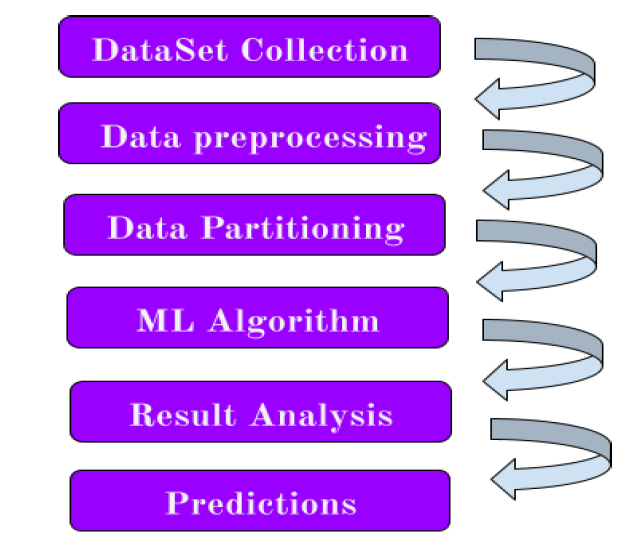
\includegraphics[width=0.8\linewidth]{fig1.png}
     \caption{ Project Flow}
 \end{figure}


\section {Dataset Description}
The Sentiment 140 dataset contains 1,600,000 tweets collected using the Twitter API. Every tweet in the dataset is annotated its polarity, indicating whether it is classified as depressed (0) or non-depressed (1), making it suitable for sentiment analysis tasks. The dataset consists of six fields:
\\
\textbf{1. target:} This field represents the polarity of the tweet, where 0 indicates a depressed sentiment and 1 indicates a non-depressed sentiment.
\\
\textbf{2. ids:} Each tweet is assigned a unique identifier (ID), facilitating easy reference and retrieval.
\\
\textbf{3. date:} This field records the date and time when the tweet was posted, providing temporal context to the data.
\\
\textbf{4. flag:} In instances where a specific query was used to extract the tweet, this field indicates the query term. If no query was used, the value is marked as NO QUERY.
\\
\textbf{5. user:} The user handle of the individual who posted the tweet is recorded in this field, offering insight into the source of the tweet.
\\
\textbf{6. text:} The text of the tweet is captured in this field, providing the actual content that was posted.
\\
The sentiment140 dataset\cite{paullada2021data}serves it serves as a particularly useful resource for training and reviewing conceptual models. detecting depressed sentiments on social media platforms like Twitter. The dataset's annotations enable researchers to explore patterns and trends in online sentiment, contributing to a deeper understanding of mental health discourse and emotional expression in digital environments. For further details on the dataset's generation and methodology, refer to the official resources provided by the creators, including the dataset link and associated paper.
\begin{table}[htbp]
    \centering
\caption{Depression Detection Dataset}
\scriptsize
 \begin{tabular}{|p{0.8cm}|c|p{2cm}|c|c|p{4cm}|}
 \hline
    \textbf{Target} & \textbf{ids} & \textbf{date}	& \textbf{flag} & \textbf{user} & \textbf{text} \\
 \hline
 0 & 1467810369 & Mon Apr 06 \newline 22:19:45 PDT \newline 2009& NO Query & TheSpecialOne & @switchfoothttp://twitpic.com 2y1zl-Awww,t.. 	\\
   \hline
1& 1467810672 &Mon Apr 06 \newline 22:19:49 PDT \newline 2009&	No Query &	scotthamilton & is upset that he cant update his Facebook by.. 	\\
\hline
2& 1467810917 & Mon Apr 06 \newline 22:19:53 PDT \newline 2009 & No Query & mattycus  & @Kenichan I divided many times for the ball.Man...	\\
\hline
3& 1467811184 & Mon Apr 06 \newline 22:19:57 PDT \newline 2009 & No Query &ElleCTF & my whole body feels itchy and like its on fire \\
\hline    
4& 1467811193&	Mon Apr 06 \newline 22:19:57 PDT \newline 2009 & No Query& Karoli& @nationwideclass no its not behaving at all... \\
\hline
     \end{tabular}
 \end{table}  
 \section {Project Procedure}
The following process is used to implement the ML model of Depression Detection.
 \begin{description}
\item[Step-1:]\textbf{Import Dependency and Dataset}

In the preliminary phase of a data-driven project, the first step entails importing essential libraries and dependencies required for subsequent analyses and model development. These libraries often include popular Python packages such as NumPy is used for numerical calculations, Pandas for data management and analysis, Matplotlib and Seaborn for data visualization, and Scikit-learn for machine learning. Additionally, depending on the project's specific requirements, other specialized libraries might be imported for tasks like deep learning (e.g., TensorFlow or PyTorch) or natural language processing (e.g., NLTK or SpaCy). 
\\
Furthermore, this step involves loading the dataset that serves as the foundation for all subsequent analyses and modeling endeavors. The dataset typically comprises structured or semi-structured data stored in various formats such as CSV files, Excel sheets, databases, or APIs. It's essential to ensure the dataset aligns closely with the project's objectives, containing relevant features and sufficient observations to facilitate meaningful analyses and model training\cite{narayanan2021efficient}. Moreover, data integrity checks may be performed at this stage to identify any anomalies or inconsistencies in the dataset that might need to be addressed during preprocessing. Overall, this initial step lays the groundwork for the entire project, setting the stage for subsequent data exploration, preprocessing, model building, and evaluation phases.
\begin{figure}[hbt!]
  \centering
  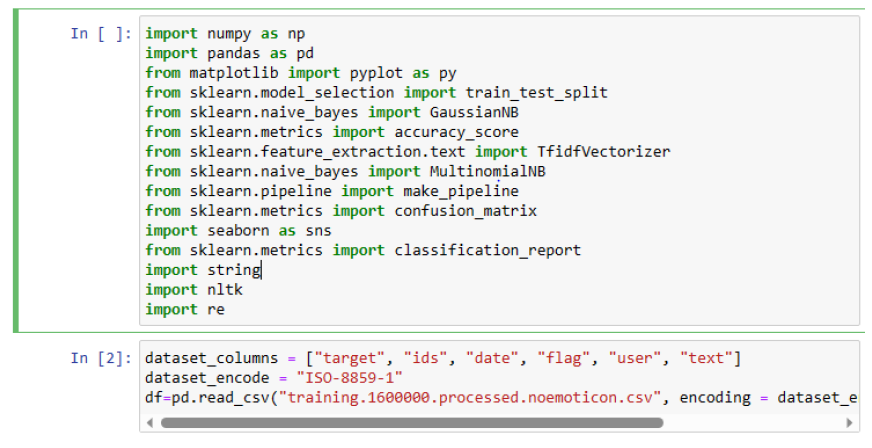
\includegraphics[width=0.6\linewidth]{C_chap/fig13.png}
\end{figure}
\\
\\
\item[Step-2:]\textbf{Data Preprocessing}

Data preprocessing is a crucial phase in any data analysis or machine learning project, where the collected dataset undergoes various transformations and enhancements to ensure its suitability for subsequent analyses and model building. This step As well as many cleaning products refining the data, addressing potential issues and inconsistencies that could hinder accurate analysis or model performance.
\\
One of the main tasks of data preprocessing is to deal with missing values. Real-world data is often incomplete or incomplete due to various reasons, such as incorrect data entry, sensor failure, or some missing data. Strategies for dealing with missing values include imputation (replacing missing values with estimates or values derived from existing data), deleting rows or columns with missing values, or using advanced techniques (such as predictive modeling) to impute missing values. values. Relationships based on data values.
\\
Another important aspect of data preprocessing involves removing duplicates, where identical or near-identical records within the dataset are identified and eliminated to avoid redundancy and ensure data integrity. Duplicate entries can skew analysis results and adversely affect model training, making their removal essential for accurate and reliable results.
\\
Additionally, categorical variables—variables that represent categories often encountered in datasets. These variables need to be encoded into numerical representations suitable for machine learning algorithms, as most algorithms operate on numerical data. Common encoding techniques include one-hot encoding, where each category is represented by a binary (0/1) indicator variable, or label encoding, where categories are replaced with numerical labels.
\\
Moreover, data preprocessing may involve scaling or normalization of numerical features to bring them within a similar range, preventing features with larger magnitudes from dominating the analysis or model training process. Standardization techniques such as z-score normalization or min-max scaling are commonly employed for this purpose.
\\
Overall, data preprocessing plays a critical role in preparing the dataset for subsequent analysis and modeling tasks, ensuring that the data is clean, consistent, and appropriately formatted for effective utilization in machine learning algorithms. By addressing issues such as missing values, duplicates, and categorical variables, data preprocessing lays the foundation for accurate insights and robust model performance, ultimately leading to more informed decision-making and actionable outcomes.
\\
\begin{figure}[hbt!]
  \centering
  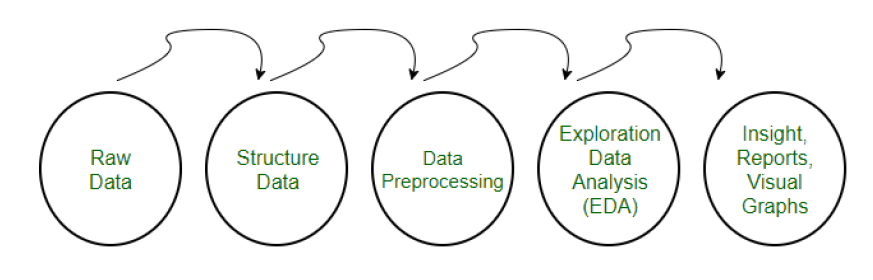
\includegraphics[width=0.8\linewidth]{C_chap/fig26.png}
\\\caption{Data Preprocessing}
\end{figure}
\\

 \begin{figure*}[hbt!]
  \centering
 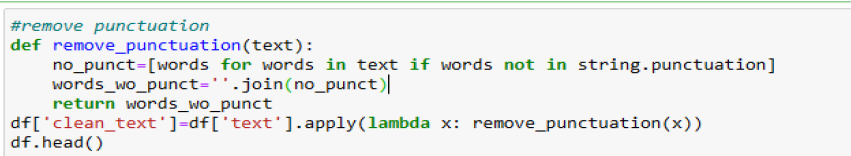
\includegraphics[width=0.8\linewidth]{C_chap/fig14.png}
\end{figure*}
 \begin{figure*}[hbt!]
  \centering
 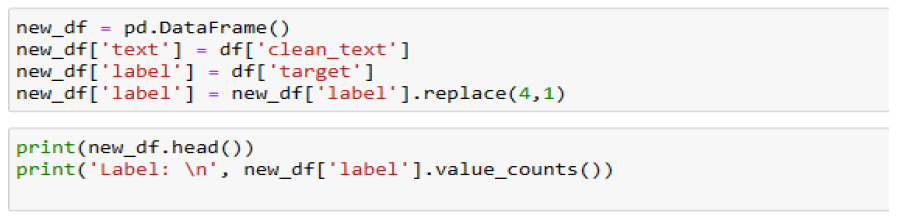
\includegraphics[width=0.8\linewidth]{C_chap/fig15.png}
\end{figure*}
\textbf{Need of Data Pre-processing: } 
Data preprocessing plays a pivotal role in ensuring the effectiveness and accuracy of machine learning models in data-driven projects. One critical aspect is aligning the data format with the requirements of specific machine learning algorithms. For instance, algorithms like Naive Bayes have strict requirements regarding data format, often not supporting null values. 
\\
Therefore, preprocessing steps such as handling missing values become essential to make the data compatible with such algorithms. Moreover, in complex projects where multiple machine learning and deep learning algorithms are employed, data preprocessing enables seamless execution and comparison across different models. By formatting the dataset appropriately and addressing issues such as outliers, scaling, and feature engineering, data preprocessing enhances the performance and speciality of machine learning models, ultimately facilitating better decision-making and insights extraction from the data.
\item[Step-3:] \textbf{Dataset Partitioning}

Dataset partitioning, often referred to as data segmentation, constitutes a pivotal phase in machine acquisition geared towards assessing the model's proficiency and effectiveness. It entails dividing the available data into distinct subsets: the training set and the testing set.
\\
The training process makes the most of the dataset and serves as the basis for teaching the learning model to recognize patterns and relationships in the data. During training, the model learns from the features and labels (if any) included in the training process. By updating its internal parameters or coefficients, the model tries to minimize the difference between its predicted properties and the actual values present in the data.
\\
Conversely, the testing set represents unseen data that the model has not encountered during the training phase. This set acts as an independent measure of the model's performance and generalization ability. through assessing the model's performance on unseen examples, we obtain understanding regarding its capacity to generate precise predictions for fresh, previously unobserved data instances. Testing methods represent real-world conditions and allow us to predict how the model will perform when used in production or when used to make predictions about future papers.
\\
The partitioning of the dataset into training and testing sets is typically performed randomly or through more sophisticated techniques such as cross-validation. The random partitioning ensures that both sets are representative of the overall dataset, reducing the risk of bias in model evaluation. Common practices dictate that a significant portion of the dataset (e.g., 70-80 Percent) is allocated to the training set, with the remainder reserved for the testing set. However, the exact split may vary depending on factors such as dataset size, complexity, and the specific objectives of the project.
\\
In summary, dataset partitioning plays a pivotal role in the machine learning workflow by enabling the assessment of model performance and generalization capability. By segregating the dataset into training and testing sets, we can train the model on one subset and evaluate its performance on another  thereby gaining valuable insights into its effectiveness and suitability for real-world applications.
 \begin{figure*}[hbt!]
  \centering
 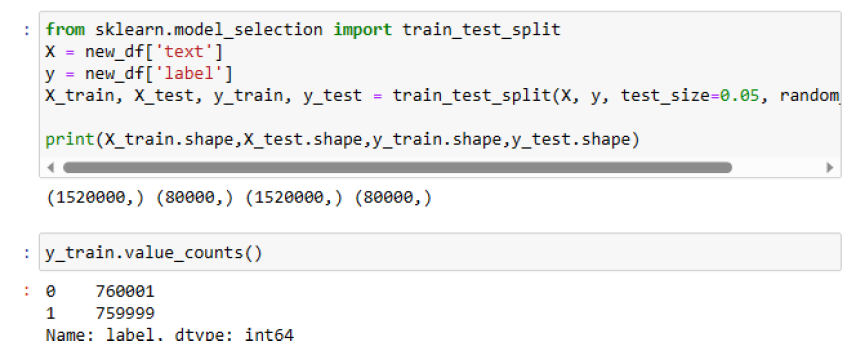
\includegraphics[width=0.7\linewidth]{C_chap/fig16.png}
\end{figure*}
%\FloatBarrier

\item[Step-4:]\textbf{ML Model}

Automated learning, a subset of Cognitive computing, empowers machines to autonomously execute tasks by learning from data samples and examples. Through the utilization of algorithms and statistical analyses, machine learning uncovers intricate patterns and correlations within datasets, often imperceptible to human observers. This capability enables machine learning models to predict outcomes, classify data, or make decisions based on new information. For instance, in natural language processing, these models adeptly comprehend the meaning and context of sentences or phrases. Likewise, in image recognition tasks, machine learning models excel at identifying and categorizing objects depicted in images. During the training phase, a machine learning model is exposed to a vast dataset, enabling it to refine its internal parameters and rules for optimal performance. As the model iteratively learns from the data, its proficiency in accurate predictions or classifications steadily improves. Ultimately, this iterative learning process culminates in the creation of a machine learning model—a sophisticated computer program equipped with tailored rules and data structures, ready to tackle designated tasks with efficiency.
\\
In supervised automated learning, models are trained using labeled data, allowing algorithms to learn patterns from input-output pairs for making predictions or classifications on unseen data. One prevalent use case of guided learning is in image recognition, where classification methods are utilized to assign images to predetermined categories or labels. Similarly, in predicting demographics such as population growth or health metrics, regression techniques are utilized to estimate continuous variables based on input features. One prominent supervised learning algorithm widely used for classification tasks is the Naive Bayes algorithm. Naive Bayes methods are grounded in Bayes' theorem, a fundamental concept in probability theory. The "naive" assumption in Naive Bayes refers to the simplifying assumption of conditional independence between every pair of features given the class variable. In other words, Naive Bayes models assume that the presence of a particular feature in a class is independent of the presence of any other feature, making the calculations simpler and more computationally efficient. Despite this simplification, Naive Bayes classifiers often perform remarkably well in practice, particularly in text classification and spam filtering tasks. By leveraging Bayes' theorem, Naive Bayes algorithms calculate the probability of a class given a set of input features, enabling them to make predictions or classifications with high accuracy and efficiency.
\\
The Multinomial Naive Bayes algorithm is a powerful Bayesian learning technique widely utilized in Natural Language Processing (NLP) tasks. Specifically designed for handling text data, this algorithm excels in tasks such as text classification, sentiment analysis, and spam filtering. In NLP, the program leverages Bayes' theorem to infer the most likely tag or category for a given piece of text, be it an email, a news article, or any other textual content. It accomplishes this by calculating the likelihood of each possible tag given the observed features (words or tokens) in the text. The algorithm then chooses the tag with a higher probability than its prediction.. This approach is particularly valuable in contexts where understanding the context or sentiment of textual content is crucial, such as analyzing customer feedback, detecting spam emails, or categorizing news articles. With the vast amount of text data available across various platforms and sources, text data classification has become increasingly essential for extracting valuable insights and making informed decisions. By accurately classifying text data, Multinomial Naive Bayes enables organizations to gain deeper insights into user perceptions, sentiments, and preferences, thereby facilitating better product development, marketing strategies, and customer engagement initiatives.
\\

 \begin{figure*}[hbt!]
  \centering
 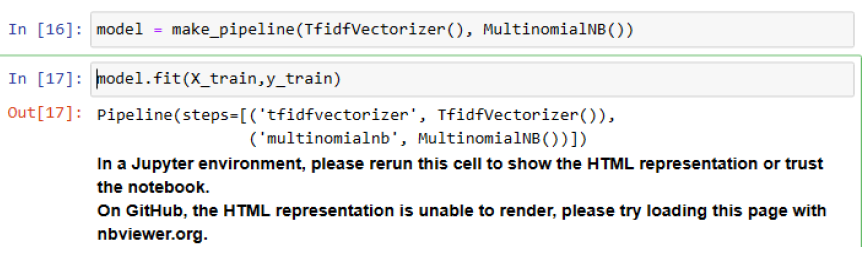
\includegraphics[width=0.8\linewidth]{C_chap/fig17.png}
\end{figure*}

\item[Step-5:] \textbf{Result Analysis}

It's crucial to assess the performance of a machine learning model after training it on data by employing distinct datasets. This evaluation phase is essential for gauging how effectively the model aligns with the data and for pinpointing any potential issues or avenues for enhancement. Utilize a range of performance metrics to scrutinize the model's proficiency in prediction or classification tasks. 
\\
These metrics may include accuracy, which measures the proportion of correctly predicted instances out of the total instances; precision, which quantifies the proportion of correctly predicted positive instances out of all instances predicted as positive; recall, which measures the proportion of correctly predicted positive instances out of all actual positive instances; and F1 score, which represents the harmonic mean of precision and recall. Other metrics such as ROC curve and AUC (Area Under the Curve) are also commonly used for evaluating models, particularly in binary classification tasks.By scrutinizing these metrics, you gain insights into the capabilities and limitations of your model. This analysis aids in fine-tuning its performance and enhancing the accuracy of its predictions. Furthermore, this evaluative procedure offers invaluable insights for iteratively refining the model, thereby bolstering its reliability and effectiveness across real-world scenarios.
 \begin{figure*}[hbt!]
  \centering
 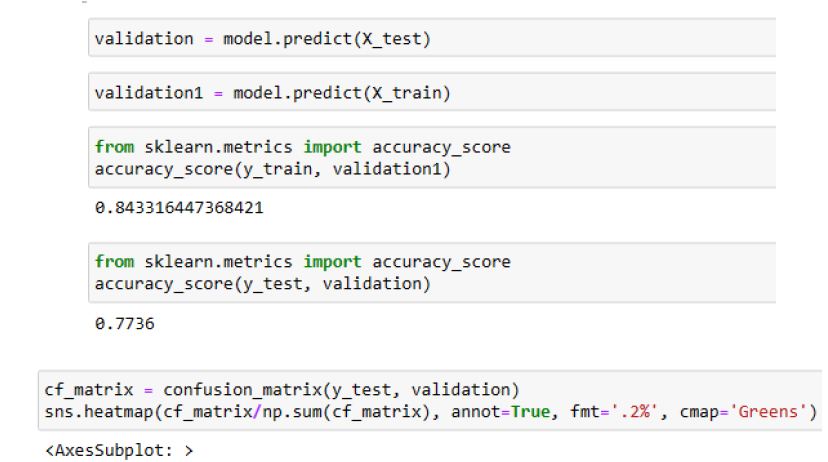
\includegraphics[width=0.8\linewidth]{C_chap/fig18.png}
\end{figure*}
 \begin{figure*}[hbt!]
  \centering
 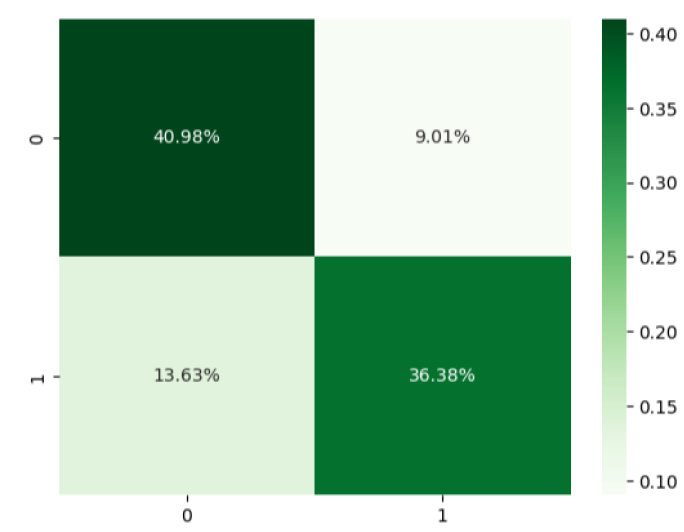
\includegraphics[width=0.8\linewidth]{C_chap/fig19.png}
\end{figure*}
 \begin{figure*}[hbt!]
  \centering
 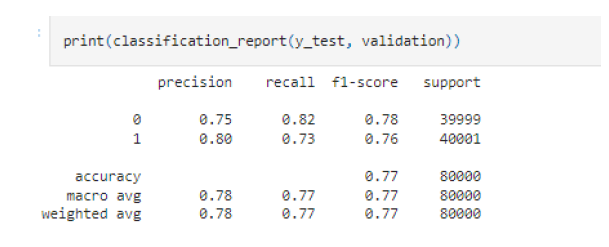
\includegraphics[width=0.8\linewidth]{C_chap/fig20.png}
\end{figure*}
\pagebreak
\item[Step-6:] \textbf{Predictions}

In the final step of the machine learning workflow, the trained model is deployed to make predictions on new, unseen data. This phase represents the culmination of the model development process, where the insights and patterns learned during the training phase are applied to real-world scenarios. Depending on the nature of the problem and the task at hand, the model may be tasked with predicting outcomes, classifying new instances into predefined categories, or clustering new data points based on similarities. Consider a predictive maintenance scenario where the model predicts potential equipment failures by monitoring sensor data for operational anomalies. Alternatively, in a customer churn prediction task, the model distinguishes between customers likely to churn and those likely to remain loyal by analyzing their behavioral patterns and demographic characteristics.
\\
 Alternatively, in a customer segmentation analysis, the model has the capability to categorize incoming customers into distinct segments according to their purchasing behaviors and preferences. Regardless of the specific application, the deployment of the trained model enables organizations to leverage the power of machine learning to drive actionable insights and make informed decisions in real-time. By continuously monitoring and updating the model with new data, organizations can ensure that it remains accurate and relevant, thus maximizing its utility and impact in addressing real-world challenges.
 \begin{figure*}[hbt!]
  \centering
 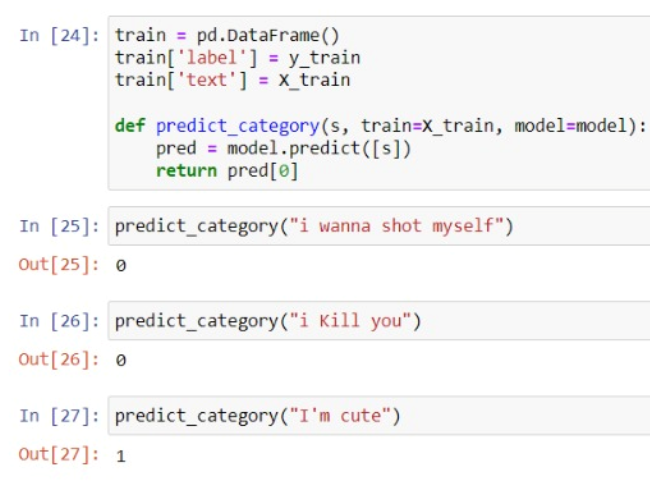
\includegraphics[width=0.8\linewidth]{C_chap/fig25.png}
\end{figure*}


\end{description}
\pagebreak
\section{ML Model} 
Machine learning stands as a foundational pillar within the broader field of artificial intelligence, enabling systems to autonomously perform tasks by analyzing vast amounts of data and examples of desired behavior. This technology not only facilitates task execution but also illuminates intricate patterns within data that may be imperceptible to human observation alone. By systematically processing and data driven learning models that learn from data can reveal relationships and patterns, thereby enriching our comprehension of complex datasets and phenomena.At its essence, a data driven learning model embodies the culmination of this learning process, equipped with the ability to discern patterns and make informed decisions when confronted with new datasets. In the realm of natural language processing, these models showcase their proficiency by deciphering the underlying intent behind previously unseen sentences, showcasing their capacity to understand the subtleties and nuances of human language. Similarly, in image recognition tasks, machine learning models are trained to accurately identify and classify objects, demonstrating their versatility and applicability across a diverse range of domains and applications.The process of training a machine learning model involves feeding it with a substantial dataset, during which the algorithm refines itself to recognize specific patterns or produce desired outputs pertinent to the task at hand. This iterative optimization imbues the model with the ability to make accurate predictions or classifications. The resultant output of this training process manifests as a computer program equipped with defined rules and data structures, forming the essence of a machine learning model.
Supervised machine learning, a prevalent paradigm in the field, entails furnishing the algorithm with an input dataset alongside corresponding desired outputs. Through this guidance, the algorithm learns to discern patterns and optimize its performance to align with the specified outputs. Classification, a technique within supervised learning, finds extensive utility in image recognition tasks, enabling models to categorize images into distinct classes. Moreover, supervised learning finds application in predicting various demographic factors such as population growth or health metrics, leveraging techniques like regression to extrapolate trends from data. This amalgamation of sophisticated algorithms and extensive datasets underscores the profound impact of supervised machine learning in diverse domains, elucidating its pivotal role in modern AI application.
\section{ML Algorithm: Naive Bayes}
Naive Bayes is a machine learning model widely used for classification tasks, particularly in scenarios with large volumes of data, including millions of records.Despite its simplicity, Naive Bayes generally produces good results, especially it is used for computational linguistics task such as emotion analysis. Recognized for its swiftness and user-friendly interface, this software offers simplicity and ease of use. Probability, in this context, denotes the likelihood of an event happening following the occurrence of another event. Bayes' theorem provides a mathematical framework for expressing this concept, enabling us to update our beliefs regarding event outcomes in light of fresh evidence.

Bayes' Theorem is represented as follows:
\begin{equation}
 P(A|B)= P(B|A)\times P(A)/P(B)   
\end{equation}
where $P(A|B)$
 is the conditional probability of event A given event B. $P(B|A)$
 is the contextual probability of event B given event A. P(A) and P(B) are the probabilities of event A and event B occurring independently.
Bayes' Theorem allows us to calculate the probability of an event A given the occurrence of event. B using prior knowledge about the probability of event 
A and the likelihood of event B given event A. This theorem is the foundation of the Naive Bayes algorithm, which applies Bayes' Theorem with the "naive" assumption of feature independence.In the context of Naive Bayes classification, Bayes' Theorem is used to calculate the probability of a class label given the features of an instance. By assuming that the features are conditionally independent given the class label, Naive Bayes simplifies the calculation of these probabilities, making it computationally efficient. Despite the simplifying assumption, Naive Bayes often performs well in practice, making it a popular choice for classification tasks, particularly in NLP applications like sentiment analysis.
The Naive Bayes Classifier operates on the principles of Bayes' theorem, making predictions based on the probabilities of data points belonging to different classes. It calculates the likelihood of each class for a given set of data and selects the class with the highest probability as the most likely outcome. This approach, also known as Maximum A Posteriori (MAP), assigns membership probabilities to each class and identifies the class with the highest probability as the optimal choice.
The MAP for a hypothesis is:
\begin{equation}
abc = abc
\end{equation}
Evidence probability, utilized for result normalization, has no impact on the outcome when removed $abc$.
In Naive Bayes classifiers, it is assumed that all variables or features are independent of each other. The presence or absence of one variable does not influence the presence or absence of any other variable.
\\
\textbf{Example:} Even when a fruit exhibits characteristics typically associated with an apple, such as being red, round, and approximately 4 inches in diameter, a Naive Bayes classifier will still assess the independence of these features to determine the likelihood of the fruit being classified as an apple.
\par
When applying our hypothesis to real datasets with numerous features, the computational complexity of our experiments increases.
\\
\textbf{Types of Naive Bayes Algorithms:}
\begin{enumerate}
    \item  \textbf{Gaussian Naive Bayes:}In Gaussian Naive Bayes, a variation of the Naive Bayes algorithm, the assumption is made that the characteristic values associated with each class follow a Gaussian or normal distribution when they are continuous in nature. This means that the distribution of these values for each class forms a bell-shaped curve, with most values clustered around the mean and fewer values spread out towards the tails of the distribution. By assuming this Gaussian distribution, the algorithm calculates the probability of observing a particular value given a class, based on the mean and standard deviation of the values for that class. This allows Gaussian Naive Bayes to effectively model the likelihood of observing certain continuous features given a class label, making it particularly suitable for datasets where the input features exhibit a continuous distribution.
\item \textbf{Multinomial Naive Bayes:} Polynomial Naive Bayes is a specially designed variant of the Naive Bayes algorithm data that follows a multinomial distribution, making it particularly well-suited for text classification tasks in natural language processing (NLP). In text classification, each document is represented as a collection of words or tokens, and the occurrence of each word in the document is considered an event. Multinomial Naive Bayes models the probability of observing a particular word given the class label, utilizing counts of word occurrences to calculate these probabilities. Since text data often exhibits a multinomial distribution, where the frequency of occurrence of words follows a discrete distribution, Multinomial Naive Bayes is widely favored for tasks such as sentiment analysis, spam detection, and document categorization in NLP. By leveraging the frequency of word occurrences in documents, Multinomial Naive Bayes effectively learns the underlying patterns in text data and enables accurate classification of documents into predefined categories or labels.
\item \textbf{Bernoulli Naive Bayes:} Bernoulli Naive Bayes is a variant of the Naive Bayes algorithm designed specifically for data that follows the multivariate Bernoulli distribution , where each feature is assumed to contain binary values. In other words, the features in the dataset are represented as binary variables, where each feature indicates the presence or absence of a particular attribute or characteristic. This variant of Naive Bayes is commonly used in scenarios where the presence or absence of certain features is crucial for classification tasks, such as document classification or spam detection. For example, in document classification, each feature may represent the presence or absence of a specific word in a document, with a value of 1 indicating its presence and 0 indicating its absence. By modeling the probability of observing each binary feature given the class label, Bernoulli Naive Bayes effectively learns the underlying patterns in the data and facilitates accurate classification based on the presence or absence of relevant features.
\end{enumerate}
\section{Deep Learning:Neural Network}
Deep learning, a subset of machine learning, harnesses the power of artificial neuron network (ANN) to learn intricate patterns and relationships present within data. Unlike traditional programming where explicit instructions are provided for every task, deep learning systems learn autonomously from data, making them adept at handling complex tasks. This approach has gained immense traction in recent years, fueled by advancements in computational capabilities and the availability of vast datasets.Hierarchical neural networks revolves around neural networks at its foundation, specifically deep neural networks (DNN), which draw inspiration from the structure and functionality of biological neurons in the human brain. These networks consist of interconnected layers of artificial neurons that process and transform input data, gradually learning to extract meaningful features and make accurate predictions. By repetitively Repair connections between neurons feedback from the data, deep learning models continually improve their performance, enabling them to tackle a wide range of tasks across various domains with remarkable accuracy and efficiency.
\\
 \begin{figure*}[hbt!]
  \centering
 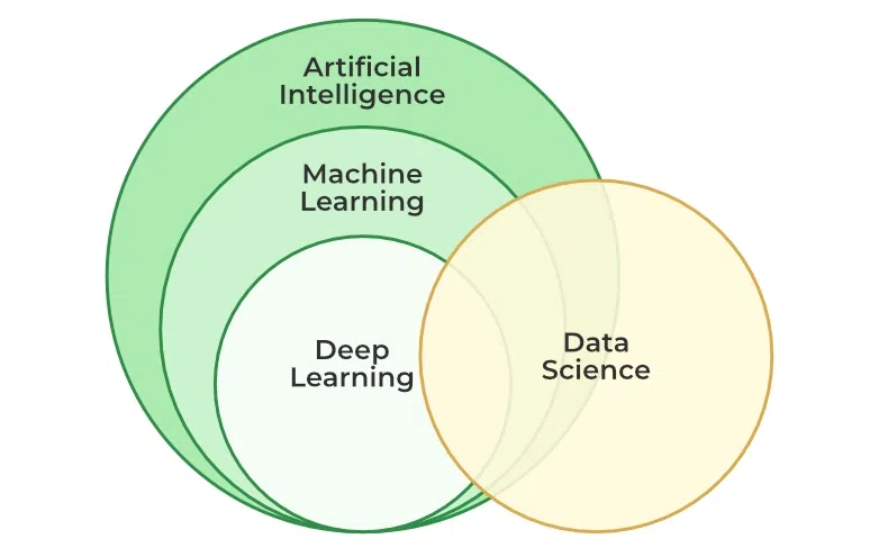
\includegraphics[width=0.8\linewidth]{C_chap/fig27.png}
     \caption{ Venn Diagram }
\end{figure*}
\\
At the heart of multi-layer learning lies the simulated network, a cornerstone concept reminiscent of the structure and functionality of human brain neural networks. These simulated networks comprise interconnected nodes known as neurons, organized into layers that typically encompass input, latent, and output processes. Within this framework, the input layer receives data, with each neuron representing a distinct feature. As data traverses through layers, intricate mathematical operations are conducted to uncover underlying patterns and correlations. The output layer generates the final outcome of the network's processing. Crucially, the connections between neurons are characterized by weights, dynamically adjusted during training via the process of Back propagation to minimize prediction errors. Activation functions introduce non-linearities, enhancing the network's capacity to comprehend complex data relationships. Through supervised learning, simulated networks iteratively refine their weights to minimize discrepancies between predicted and actual outputs, facilitating the ability to generalize and make accurate predictions on new data instances. This adaptability and adeptness at discerning subtle patterns render simulated networks indispensable for a myriad of tasks, including image recognition, natural language processing, and speech recognition, propelling advancements in artificial intelligence and machine learning.
\subsection{Artificial Neural Network}
The intricacy of a neural network is contingent upon the underlying data patterns and the myriad processes it undergoes, ranging from a few to potentially millions. Typically, a neural network comprises an input layer, one or more hidden layers, and an output layer. The ingress process sources information from various origins such as external devices, network analysis, or learning mechanisms. Subsequently, data traverses through layers, undergoing transformations to extract pertinent insights for subsequent processing. Each unit within the hidden layer receives input from preceding layer neurons, computes the weighted sum of these inputs, and applies a function to generate an output signal. The interconnections between units are governed by corresponding weights, dictating the influence of one unit's output on another. Throughout training, these weights are continually adjusted to optimize network performance. Ultimately, the egress process generates a response based on the processed input data. Drawing inspiration from human neuron structures and functions, this iterative process empowers artificial neural networks to glean knowledge from data and make accurate predictions or classifications.
\\
In a neural network, Nodes, also called neurons, are arranged in layers typically consisting of three main layers: the input layer, the hidden layer(s), and the output layer.
\\
\textbf{1. Input Layer:} The input layer is where the neural network receives its initial input data. Each node in this layer represents a feature or attribute of the input data. For example, in an image recognition task, each node might represent a pixel value in the image. The input layer serves to pass the input data to the subsequent layers for processing.
\\
\textbf{2. Hidden Layer(s):} Situated between the input and output layers, the hidden layer(s) act as transitional components within the neural network structure. Their core role entails performing a series of mathematical computations to efficiently handle the input data. Each node in the hidden layer(s) receives input from every node in the previous layer and applies a transformation to generate its output. The number of hidden layers and the number of nodes in each hidden layer can vary depending on the complexity of the problem and the desired model architecture. Hidden layers enable the neural network to learn complex patterns and relationships within the data by extracting relevant features.
\\
\textbf{3. Output Layer:} The output layer is the final layer of the neural network, where it produces the desired output or prediction. Each node in the output layer represents a class or category that the model aims to classify or predict. The output layer's size and structure depend on the nature of the task. For instance, in a binary classification problem, there may be two nodes representing the two possible classes, while in a regression problem, there might be a single node representing the continuous output value.
\\
 \begin{figure*}[hbt!]
  \centering
 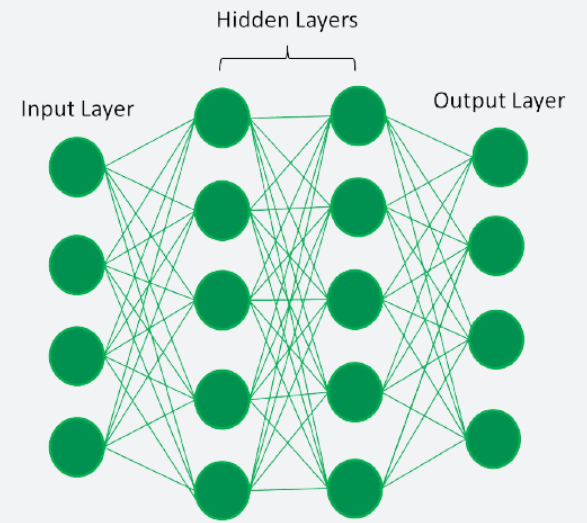
\includegraphics[width=0.8\linewidth]{C_chap/fig28.png}
     \caption{Fully Connected Artificial Neural Network }
\end{figure*}
\\
Overall, the arrangement of nodes in these three layers forms the foundation of a neural network's architecture. Through training, which involves adjusting the parameters (weights and biases) of the connections between nodes, the neural network learns to map input data to the desired output, making it capable of performing various tasks such as classification, regression, and pattern recognition.
\subsection{Artificial Neuron vs Biological Neurons}
Artificial neural networks (ANN) are computational models inspired by the biological nervous system, particularly the structure and function of neurons in the brain. These networks consist of interconnected nodes, or artificial neurons, arranged in layers.
\\
\textbf{Structure:} Biological neurons have a cell body that integrates incoming signals from dendrites, processes them, and generates output signals along the axon. In ANN, input nodes receive input signals from external sources, which are then transmitted through weighted connections to hidden layer nodes. The hidden layer nodes process these signals using activation functions and pass them to output layer nodes, which produce the final output of the network.
\begin{table}[htbp]
   \centering
\caption{Biological vs Artificial Neuron}
\scriptsize
 \begin{tabular}{|p{3cm}|p{2cm}|}
 \hline
   \textbf{Biological Neuron} & \textbf{Artifical Neuron} \\
\hline
Dendrite & Input \\
\hline
Cell nucleus or soma & Nodes  \\
\hline
Synapses & Weights \\
\hline
Axon & Output  \\
\hline
Synaptic Plasticity & Backpropogation \\
\hline
    \end{tabular}
  \end{table}


\textbf{Synapses:}
Synapses are the connections between neurons in the brain, where neurotransmitters are released to transmit signals from one neuron to another. In ANN, synapses are represented by the weighted connections between nodes in adjacent layers. These weights determine the strength of the connection between nodes and are adjusted during the training process to optimize the network's performance.
\\
\textbf{Learning:} In biological neurons, learning occurs through synaptic plasticity, which involves strengthening or weakening of synaptic connections in response to neural activity. Similarly, in ANN, Learning is facilitated through training algorithms like backpropagation, which iteratively fine-tune the weights of connections between nodes by assessing the disparity between predicted and observed output values. This iterative process enables the network to glean insights from input-output pairs, progressively enhancing its performance over successive iterations.
\\
\textbf{Activation:} Activation refers to the process by which neurons become active and transmit signals to other neurons. In biological neurons, activation occurs when the membrane potential reaches a certain threshold, triggering an action potential. In ANN, The activation function determines the output of the node based on the weight of the inputs. Common functions include sigmoid, tanh, ReLU (rectified linear unit), etc. and each of them has its own characteristics and uses. in different types of networks.
\\
Overall, ANNs emulate the structure and function of biological neurons to perform various computational tasks, including pattern recognition, classification, and regression. By learning from data and adjusting their internal parameters, neural networks can adapt to complex input-output relationships and Make predictions or decisions based on sample data.
\\
 \begin{figure*}[hbt!]
  \centering
 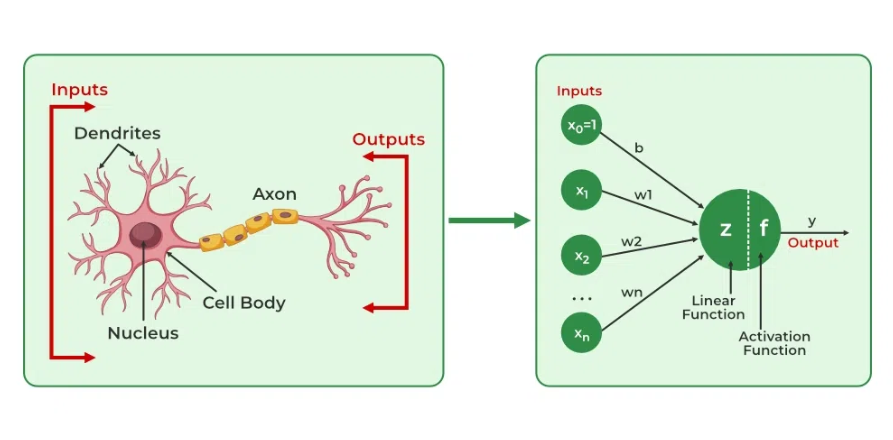
\includegraphics[width=0.9\linewidth]{C_chap/fig29.png}
     \caption{Biological neurons to Artificial neurons }
\end{figure*}
\subsection{Learning of ANN}
Artificial neural networks (ANN) are trained using a process called supervised learning, where they learn from labeled training data. In the example provided, let's consider training an ANN to recognize images of cats. The training process involves presenting the ANN with thousands of different images of cats, along with corresponding labels indicating that they are indeed images of cats.
\\
During training, the ANN processes each image through its layers of interconnected nodes, with the input layer receiving pixel values from the image and passing them through the network. As the data propagates through the network, Adjust the weight of the connection between nodes based on the difference between predicted and actual results provided in the training data.
\\
Once the ANN has been trained using a sufficient amount of cat images, it needs to be evaluated to determine its performance in correctly identifying cat images. This evaluation involves presenting the ANN with a new set of images, both cat images and images of other objects or scenes, and observing its classification decisions.
\\
If the ANN fails to classify an image (i.e., it incorrectly identifies a non-cat image as a cat, or vice versa), back propagation is used to update the network's weights and biases. Back propagation involves Calculate the error, or loss, between the estimated output and the actual tag, and then propagate this error backwards through the network to adjust the weight and bias of the link to minimize errors.
\\
This process of presenting data, calculating errors, and adjusting weights is repeated repetitively until the ANN achieves a satisfactory level of performance, typically measured by metrics such as accuracy or error rate. Through this iterative learning process, the ANN gradually learns to Identify specific patterns and features in cat images, allowing it to make accurate predictions on unseen data.
\\
Overall, training an ANN involves exposing it to a large amount of labeled data, fine-tuning its parameters through back propagation, and repetitively refining its performance until it achieves the desired level of accuracy in classification tasks.
\section{Algorithm:Convolution Neural Network}
A Convolution Neural Network (CNN) is a type of deep learning algorithm primarily used for image recognition and classification tasks. CNN are inspired by the biologicalVisual cortex designed to automatically learn spatial hierarchies of features from input data \cite{wang2020cnn}.

Here's a simplified explanation of how CNN work:
Sure, let's dive deeper into each component of a Convolution Neural Network (CNN) and how they work:

\textbf{1. Convolution Layers:}
In convolution layers, Convolution Neural Networks (CNN) apply convolution Filter (also called kernel) data input. These filters are small matrices that slide over the input image, providing equal content and ensuring equal processing of each function. Each filter is designed to detect specific patterns or features in objects, such as edges, textures, or shapes. For instance, one filter might be sensitive to vertical edges, while another is tuned to detect horizontal edges. As the filters convolve across the input image, they generate feature maps that highlight the presence of different features. Each feature map represents the response of the corresponding filter to the input image and serves as a higher-level representation of the input data, capturing important visual patterns and structures. Through the learning process, CNN adjust the weights of these filters to effectively extract meaningful features from the input data, enabling them to perform tasks such as image classification and object detection.
\\
  

\textbf{2. Activation Function (ReLU):}
After the convolution operation in a Convolution Neural Network (CNN), an activation function is applied element-wise to introduce non-linearity into the model. This step is essential because it allows the network to capture complex relationships and patterns within the data, which may not be effectively represented by linear transformations alone. One of the most commonly used activation functions in CNN is the Rectified Linear Unit (ReLU). ReLU applies a simple mathematical operation to each element of the feature map, replacing any negative pixel values with zero while leaving positive values unchanged. This non-linear transformation enables the network to model more intricate features and interactions, improving its ability to learn and generalize from the input data. By introducing non-linearity through activation functions like ReLU, CNN can effectively handle the complexities of Functions such as image recognition, target detection and semantic classification, leading to improved performance and accuracy.
\\

\textbf{3. Pooling Layers:}
Pooling layers in Convolution Neural Networks (CNNs) serve the crucial role of reducing the width of the map while keeping the information simple. This area reduction is achieved by a function such as maximum pooling, which is a maximum pooling technique. During maximum pooling, a small window (usually 2x2 or 3x3) is shifted across the feature map and the maximum value in each window is retained while other values are discarded. By preserving only the maximum activation within each window, max-pooling effectively compress the feature maps, reducing computational complexity and memory requirements. Additionally, it aids in controlling training by enforcing spatial steady and promoting the detection of robust features across different regions of the input data. Overall, pooling layers play a critical role in extracting salient features from the input data while simultaneously reducing its spatial resolution, thereby facilitating efficient and effective feature extraction in CNN.


\textbf{4. Flattening:}
In the process of building a Convolution Neural Network (CNN), after multiple convolution and pooling layers, the resulting feature maps are flattened into a one-dimensional vector. This step, known as flattening, is essential for preparing the data to be input into a fully connected neural network (FCNN). By flattening the feature maps, the spatial information captured during the convolution and pooling operations is converted into a linear format. This transformation is necessary because fully connected layers require one-dimensional input vectors. Flattening essentially collapses the multi-dimensional feature maps into a single continuous vector, where each element represents a specific feature or activation. This linear representation enables the subsequent fully connected layers to learn complex relationships between the extracted features and the target classes during the classification process. Overall, the flattening stage serves as a critical bridge between the convolution layers responsible for feature extraction and the fully connected layers responsible for classification, facilitating the seamless flow of information through the CNN architecture.
\\

\textbf{5. Fully Connected Layers:}
 In the Convolution Neural Network (CNN) architecture, the flattened feature vector, obtained after the convolution and pooling layers, is fed into One or more layers, also called thick layers. All these layers play an important role in the classification process of learning intricate relationships between the extracted features and the target classes. Each neuron in the fully connected layer is connected to every neuron in the previous layer, enabling the network to capture high-level representations of the input data. Through this dense interconnection, the fully connected layers can effectively Learn and model complex patterns and dependencies found in data. Adjust weights and biases iteratively training process, these layers refine their parameters to optimize the classification accuracy, ultimately enabling the CNN to make accurate predictions on unseen data. Overall, the fully connected layers serve as the decision-making component of the CNN, where the learned features are transformed into predictions or classifications based on the network's learned parameters.
\\

\textbf{6. Output Layer:}
In convolutional neural network (CNN) architecture, the output layer serves as the final step in building the prediction network. It usually consists of one or more neurons, and each neuron corresponds to a group in the classification function. The number of neurons in the output layer matches the number of groups the CNN is designed to distribute. Different processes are used in the output layer depending on the nature of the job. For various classification functions, softmax initial functions are often used, which convert the scores of the raw data of each category into probabilities to ensure that the probability of each category equals 1. In contrast, in binary classification, a sigmoid activation function is used to make each class independent. The output value produced by the output method represents the probability estimate for each class, allowing the CNN to make informed decisions about classifying the input data according to the highest level. The latter process plays an important role in determining the overall performance of the network and its ability to analyze incoming data into its categories.

\textbf{7. Training:}
Training a convolutional neural network (CNN) involves an iterative process of replacing a network failure to minimize performance loss. This process is caused by a process called backpropagation; where the error between the output estimate and the ground truth map is propagated back through the network, allowing for the slope of the loss function with respect to the network parameters. Optimization algorithms such as gradient descent are then used to adjust the weight and bias of the convolution filters and all layers in the network, thus gradually reducing the loss and improving the tuning of the network performance. The goal is to make the predicted output as close as possible to the real text in the training data, thus effectively learning underlying patterns and relationships in objects. Thanks to this training process, CNN learns the hierarchical representation of visual data, allowing it to perform many tasks such as image classification, target detection and image segmentation accurately and effectively.
\\
 \begin{figure*}[hbt!]
  \centering
 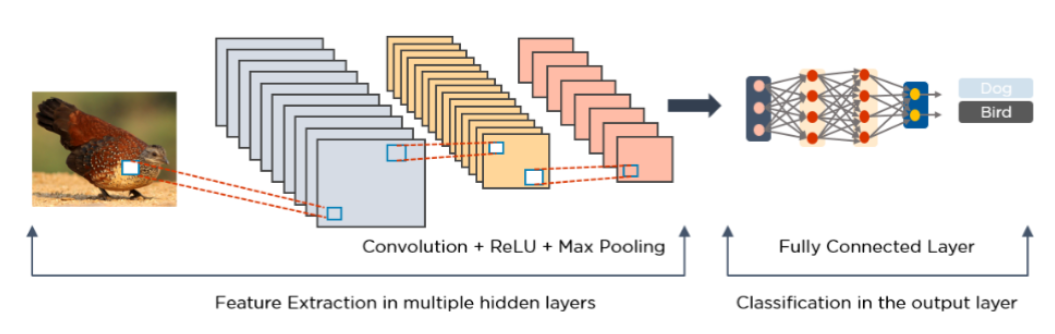
\includegraphics[width=0.9\linewidth]{C_chap/fig30.png}
     \caption{Image Processed via CNN}
\end{figure*}
\\
Overall, CNN excel at learning spatial hierarchies of features from input data, making them well-suited for a wide range of computer vision tasks.
\section{Data Set Description:Audio Sentiment Recognition}
The Ryerson Audio-Visual Database of Emotional Speech and Song (RAVDESS) stands as a cornerstone resource for researchers delving into the intricate realm of emotional expression, particularly within the domains of speech and song. Boasting contributions from 24 seasoned actors, evenly divided between genders, RAVDESS offers a rich tapestry of vocal performances encompassing a diverse array of emotions. From the subtle tranquility of calm to the explosive intensity of anger, from the infectious joy of happiness to the haunting depths of sadness, the dataset encapsulates the full spectrum of human emotional experience.
\\
One of the standout features of RAVDESS is its meticulous attention to emotional nuance. Each emotional expression is not only meticulously crafted but also presented at two distinct levels of intensity: normal and strong. This nuanced approach allows researchers to probe deeper into the intricate interplay between emotional states and vocal cues, shedding light on the subtle nuances that underpin human communication and perception.
\\
Furthermore, RAVDESS offers researchers the flexibility to explore these emotional expressions across different modalities. Whether researchers seek to dissect the acoustic subtleties of speech, dissect the visual cues embedded in audio-video recordings, or solely focus on the visual aspects through video-only files, RAVDESS accommodates a wide range of experimental designs and analytical approaches.
\\
The organizational structure of the dataset also merits praise for its clarity and efficiency. With files neatly organized into folders corresponding to individual actors, researchers can easily navigate through the wealth of data. Each file follows a standardized naming convention, providing detailed information about the modality, vocal channel, specific emotion, intensity level, statement, repetition, and actor involved. This meticulous labeling system streamlines data management and retrieval, ensuring researchers can swiftly locate and utilize the relevant data for their experiments.
\\
Despite its many strengths, it's essential to acknowledge the limitations of this dataset. Actor number 18 notably lacks song version data, and certain emotions such as disgust, neutral, and surprised are absent from the song version recordings. Researchers must take these limitations into account when designing experiments and interpreting results to ensure the integrity and validity of their findings.
\\
The dataset represents a treasure trove of invaluable resources for researchers venturing into the multifaceted realm of emotional expression. Its comprehensive coverage, nuanced emotional portrayals, versatile modalities, and meticulous organization make it an indispensable tool for advancing our understanding of human communication, perception, and cognition across a myriad of academic and commercial endeavors.
\\
\section{Project Flow of Audio based Depression Detection}
The project flow for speech emotion recognition using Convolution Neural Network (CNN) entails a systematic process of analyzing audio data to discern emotional states. It begins with the provision of voice data in .wav format, which is then meticulously read and processed to extract relevant features. These features are visualized through waveform or spectrogram plots, aiding in understanding the underlying patterns within the audio signals. Subsequently, the dataset undergoes partitioning into training and testing subsets, facilitating the evaluation of the CNN model's performance. The CNN model is meticulously crafted and trained on the training data, enabling it to autonomously learn and extract salient features crucial for identifying emotions from speech. Post-training, the model is deployed to predict emotions or sentiments on the test data, which are then compared against ground truth labels using array sequences, thus quantitatively assessing the model's efficacy. The culmination of this process yields insights into the emotional state of the speaker, discerning whether they are stressed or not. Leveraging the capabilities of deep learning, the CNN model adeptly interprets emotional cues embedded within speech signals, thereby offering invaluable implications for diverse applications such as mental health monitoring and enhanced human-computer interaction paradigms.
\\
 \begin{figure*}[hbt!]
  \centering
 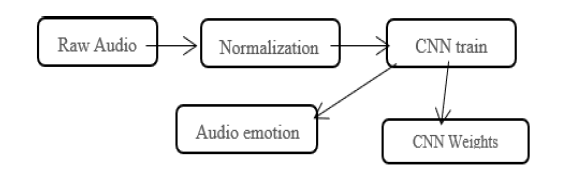
\includegraphics[width=0.8\linewidth]{C_chap/fig36.png}
     \caption{Project Flow of CNN Model}
\end{figure*}
\\
The following process is used to implement the speech emotion recognition model of Depression Detection.
\\
\textbf{Step 1: Data Collection and Preprocessing}
\\
The data collection and pre processing steps involved in developing an emotion recognition system using audio recordings. The dataset used comprises recordings from various actors expressing different emotions. Prior to model training, the raw audio files undergo pre processing to extract Mel-frequency cepstral coefficients (MFCCs), which capture essential acoustic information while reducing extensity. Each audio sample is labeled with specific emotion categories such as anger, calmness, fear, happiness, or sadness, enabling supervised learning. This annotation schema facilitates the model's ability to learn patterns between acoustic features and emotional states. Overall, these preparatory steps lay the foundation for subsequent model training and evaluation, enhancing the system's accuracy in discerning emotions from real-world audio data.
\\
 \begin{figure*}[hbt!]
  \centering
 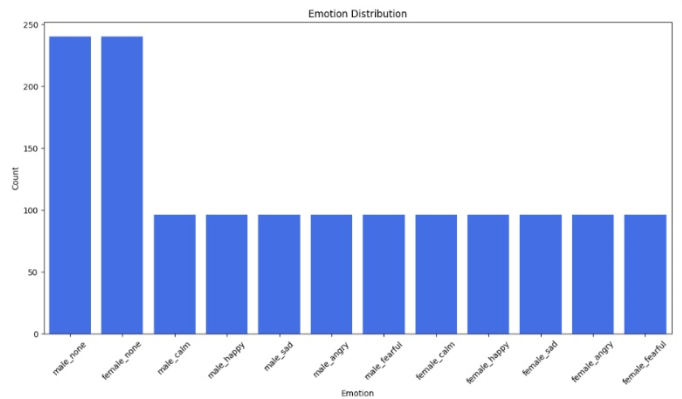
\includegraphics[width=0.9\linewidth]{C_chap/fig32.png}
     \caption{Emotion Distribution}
\end{figure*}
\\
\textbf{Step 2: Data Analysis and Visualization}
\\
In the realm of audio emotion recognition system development, data analysis and visualization play a pivotal role in understanding the dataset's characteristics and underlying patterns. By employing various techniques, analysts gain insights into the distribution of emotions within the dataset, using visualizations like bar charts to depict the prevalence of different emotional states. This analysis ensures the model is trained on a diverse and representative set of examples. Moreover, visualizing waveform and spectrogram provides a deeper understanding of the audio data temporal and spectral properties, aiding in the identification of patterns indicative of different emotional states. Through thorough data analysis and visualization, researchers can uncover valuable insights, facilitating model development, evaluation, and the interpretation of predictions. Ultimately, this comprehensive understanding of the data enhances the robustness and accuracy of audio emotion recognition systems.
\\
 \begin{figure*}[hbt!]
  \centering
 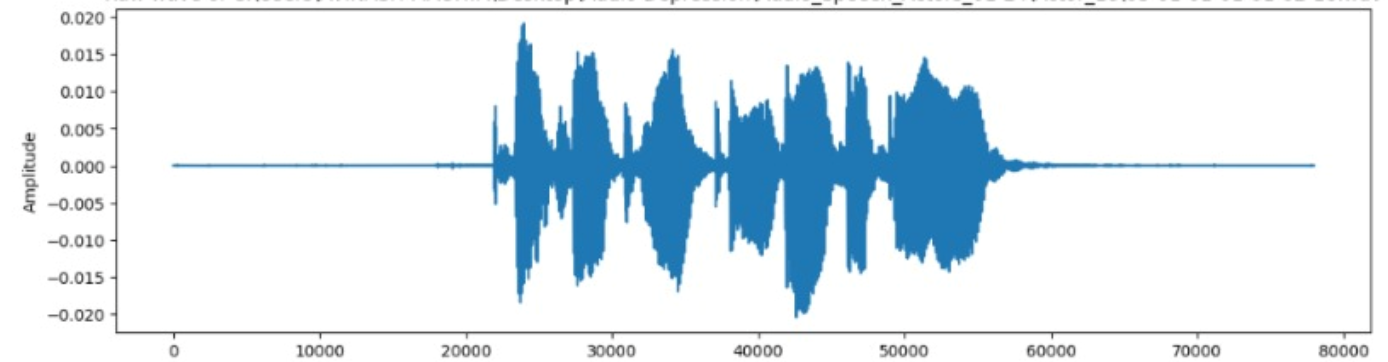
\includegraphics[width=0.9\linewidth]{C_chap/fig33.png}
     \caption{Amplitude Plot of Raw wave}
\end{figure*}
\\
 \begin{figure*}[hbt!]
  \centering
 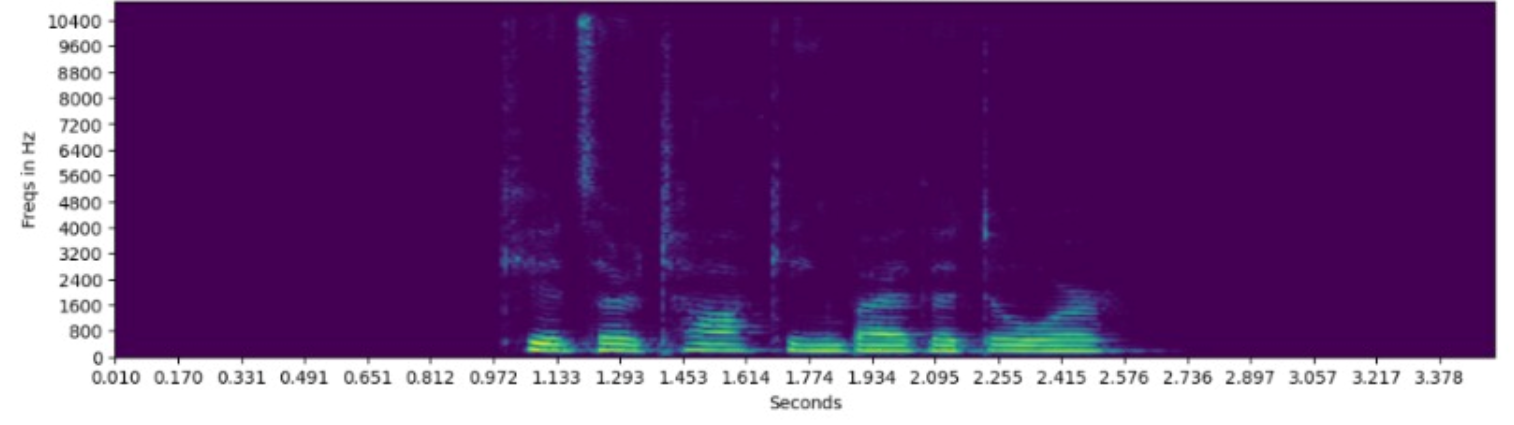
\includegraphics[width=0.9\linewidth]{C_chap/fig34.png}
     \caption{Spectrogram Plot}
\end{figure*}
\\
\textbf{Step 3: Data Augmentation}
\\
In the pursuit of fortifying the robustness and generalization capabilities of the audio emotion recognition system, data augmentation proves to be a crucial strategy. This process involves introducing variations and perturbations to the existing audio recordings through a suite of techniques such as noise addition, shifting, stretching, and pitch tuning. By augmenting the training dataset in this manner, the model becomes more adept at discerning emotional cues amidst varying levels of background interference, simulating real-world scenarios where environmental noise may obscure the underlying emotional expression. Moreover, temporal manipulations like shifting and stretching introduce variations in speech tempo and rhythm, enabling the model to generalize effectively across different speaking styles. Additionally, pitch tuning exposes the model to a spectrum of pitch variations, enhancing its understanding of the acoustic features associated with different emotional states. Overall, data augmentation enriches the training dataset with greater diversity and complexity, empowering the model to excel in diverse real-world environments characterized by noise, variability, and nuance. Through judicious application, data augmentation enhances the system's capacity for accurate emotion recognition, ensuring its resilience and adaptability across a wide range of scenarios.
\\
\textbf{Step 4: Model Architecture}
\\
At the core of the audio emotion recognition system lies a meticulously crafted model architecture built upon the foundational principles of Convolution Neural Networks (CNN). This architecture is designed to distill complex audio features into discernible emotional categories through a hierarchical structure. Beginning with convolution layers, strategically positioned to convolute over spectrogram representations of the audio data, the model extracts salient temporal and frequency patterns indicative of emotional nuances. Pooling layers then compress these features, capturing their spatial hierarchies while reducing computational complexity. Dense layers follow, consolidating hierarchical representations into compact feature vectors amenable to emotion classification through non-linear transformations. Dropout layers are strategically integrated to mitigate training by uncertainly deactivating neurons during training. Upon construction, the model undergoes compilation, utilizing categorical cross-entropy loss and the Adam optimizer to quantify prediction disparities and optimize parameters, respectively, thereby enhancing classification accuracy and convergence speed. This meticulously engineered architecture enables the system to discern subtle emotional distinctions encoded within audio data while ensuring robustness and generalization across diverse emotional expressions.
\\
\textbf{Step 5: Model Training}
\\
Model training constitutes the life-changing crucible where neural networks undergo iterative refinement, assimilating the intricacies of training data to become adept classifiers of emotional states within audio recordings. This process initiates with dataset partitioning into training and validation subsets, facilitating performance evaluation on unseen data. Amidst epochs of training, the model refines its parameters repetitively to minimize loss and maximize accuracy. Key interventions, orchestrated by callbacks, augment training efficacy and resilience. Model control unit ensures the preservation of optimal configurations, while learning rate reduction mechanisms dynamically navigate optimization landscapes. Metrics like loss and accuracy serve as performance barometers, guiding model architects towards iterative improvements in architecture and training protocols for superior classification outcomes. Through vigilant monitoring and adaptation, the model evolves to adeptly capture emotional dynamics within audio data, contributing to its efficacy in real-world applications.
\\
\textbf{Step 6: Model evaluation}
\\
During the model's evaluation on the test dataset, various performance metrics such as accuracy and F1-score are utilized to gauge its effectiveness in classifying emotions within audio recordings. These metrics provide a comprehensive assessment of the model's capabilities, while the confusion matrix offers a nuanced view of its classification prowess across different emotions. By analyzing the matrix, evaluators identify areas of strength and weakness, guiding future refinements and improvements. Ultimately, the evaluation serves as a catalyst for continued exploration and advancement in audio emotion recognition, empowering researchers to delve deeper into this complex domain armed with valuable insights gleaned from rigorous evaluation processes.
\\
\textbf{Step 7: Deployment and Testing}
\\
After the rigorous training process, the model is ready for deployment, marking the culmination of its development journey. Serialized for seamless integration into various environments, the model is tested with real-world audio files to evaluate its ability to recognize emotions accurately amidst everyday noise. Through iterative testing and refinement, the model adapts to diverse scenarios, enhancing its discernment and robustness. Deployment signifies not just the end of one phase but the beginning of another, as developers continually refine the model based on real-world feedback, ensuring its evolution into a dynamic tool for emotion recognition in various contexts.
\section{Real Time ECG Monitoring}
The article highlights the significance of mental health, particularly focusing on depression as a widespread condition impacting millions worldwide. It underscores the importance of early detection and intervention for effective treatment. Traditional approaches, such as self-reporting and clinical assessments, are acknowledged for their subjectivity and time-consuming nature. To address these challenges, the article introduces an innovative approach leveraging wearable technology and machine learning to transform depression detection. This novel method aims to provide a more objective and efficient means of identifying individuals at risk of depression, potentially revolutionizing the way mental health conditions are diagnosed and managed \cite{Krishnan2018iot} .
\\
The project introduces a hardware device crafted with an ESP8266 microcontroller \cite{schwartz2016internet} and an AD8232 sensor, designed to provide a non-invasive wearable solution. This wearable can be easily worn by users and operates by continuously monitoring their heart rate data. The collected physiological data is then transmitted without wire, potentially to a cloud-based platform, for in-depth analysis. This real-time monitoring offers a unique insight into the user's well-being, providing a continuous stream of physiological information. Such data could unveil subtle patterns and trends that traditional assessment methods might overlook, potentially offering valuable insights into the user's overall health status and aiding in early detection and intervention for conditions like depression.
\\
The project extends beyond mere data collection by proposing the utilization of machine learning algorithms to analyze the heart rate information gathered by the wearable device. Machine learning, renowned for its ability to discern intricate patterns and correlations within complex datasets, is identified as a potent tool for this task. By applying these advanced algorithms to the collected heart rate data, the project aims to develop a sophisticated system capable of detecting potential indicators of depression. Through the analysis of subtle variations and trends in heart rate patterns, the system seeks to identify early signs of depressive symptoms. This early detection holds immense potential in facilitating timely intervention and treatment, enabling healthcare professionals to offer support and assistance to individuals at risk of depression before their condition exacerbates, ultimately improving patient outcomes and well-being.
\\
The potential benefits of this project extend far beyond the realm of individual patients, impacting both healthcare outcomes and system efficiency. Early and precise detection of depression holds the promise of vastly improving patient outcomes by enabling timely intervention and treatment initiation. By identifying individuals at risk of depression at an early stage, healthcare professionals can intervene promptly, potentially preventing the condition from escalating and leading to more severe consequences. Moreover, this approach has the potential to alleviate the burden on healthcare systems by facilitating remote monitoring and early intervention. Through continuous monitoring of physiological data via wearable technology, healthcare providers can proactively identify and support individuals at risk, reducing the need for extensive clinical assessments and hospital visits. This not only improves patient care but also optimizes resource allocation within healthcare systems, ultimately enhancing overall system efficiency and effectiveness.
\\
In conclusion, this project represents a major advance in depression research, leveraging the combined power of wearable technology and machine learning. Through continuous monitoring of heart rate data and the application of sophisticated algorithms, the project endeavors to achieve early and precise diagnosis of depression. The potential implications of this approach are profound, with the promise of improving patient outcomes by enabling timely intervention and treatment initiation. Moreover, the project has the potential to alleviate the burden on healthcare systems by enabling remote monitoring and early intervention, thereby optimizing resource allocation and enhancing overall system efficiency. The upcoming sections of the project will provide a detailed exploration of the technical aspects of the device, the machine learning methodology employed, and the broader implications for the field of mental health, shedding light on the life changing potential of this innovative approach.
\\
\section{Hardware and Methods}
The project aimed at designing a heart monitoring system tailored to different weight categories of subjects, there are two crucial stages essential for achieving the proposed objective. Firstly, the sensing, processing, and display units must seamlessly collaborate to ensure the efficient functioning of the system. The heart electrical activities sensor, which outputs digital data, plays a pivotal role in sensing the physiological signals. This sensor's output can be seamlessly integrated with any of the digital pins of the Nodemcu microcontroller, facilitating communication between the sensor and the Nodemcu unit. This integration forms the foundational step in the data acquisition process, allowing the system to capture and process the heart's electrical signals effectively.
Secondly, the communication aspect between the Nodemcu unit and the Ubidots \cite{mohammed2021real} software is paramount for transmitting the collected data to the intended recipient, such as the patient's phone. Ubidots serves as the intermediary platform for this communication, enabling seamless data transfer and visualization for the patient's monitoring. The ESP8266 board, equipped with specific pins designated for transmission and reception of data, facilitates the communication interface between the Nodemcu unit and the Ubidots software. Through this synchronized communication setup, the system ensures real-time monitoring and tracking of the patient's heart activity, thereby contributing to enhanced healthcare management and patient well-being.
\\
\textbf{Stage 1 : Sensing}
\\
In the sensing stage of the heart monitoring system project, the primary objective is to capture the electrical activities of the heart using appropriate sensors. The chosen sensor for this project outputs a digital signal, which implies that it provides data in a digital format rather than analog. This digital output simplifies the interfacing process with the Nodemcu board, as digital signals are easier to handle and process within digital electronic systems.The digital output from the sensor can be seamlessly connected to any of the digital pins available on the Nodemcu board. These digital pins are versatile and can be configured to either read digital inputs or provide digital outputs, depending on the requirements of the system. By connecting the sensor's digital output to one of these pins, the Nodemcu board can effectively capture the heart's electrical activities in a format that is compatible with its digital processing capabilities.This integration of the sensor's digital output with the Nodemcu board forms the foundation of the sensing stage, enabling the system to accurately capture and process the heart's electrical signals. Through this setup, the system can gather essential physiological data necessary for monitoring the patient's heart health and facilitating further analysis or action as needed.
\\

\textbf{Stage 2: Processing and Display}
\\
\textbf{2.1 Nodemcu Integration:} In the heart monitoring system project, the Nodemcu board plays a pivotal role in integrating various components and facilitating communication between them. As a versatile microcontroller board based on the ESP8266 chip, the Nodemcu offers the necessary computational power and connectivity features required for this application. One of its primary functions in this project is to receive data from the heart sensor and relay it for further processing and transmission.The digital output from the heart sensor, which captures the electrical activities of the heart, is seamlessly connected to one of the digital pins on the Nodemcu board. These digital pins serve as the interface through which the Nodemcu communicates with external devices or sensors. By connecting the sensor's digital output to one of these pins, the Nodemcu establishes a direct pathway for receiving the heart signal data in digital format.
Once the sensor's digital output is connected to a digital pin on the Nodemcu, the microcontroller can effectively receive and process the incoming data. This integration enables the Nodemcu to capture the heart's electrical activities in real-time, paving the way for further analysis or transmission as required by the project objectives. Through this seamless integration, the Nodemcu acts as a central hub for data acquisition, enabling the heart monitoring system to function efficiently and effectively.
\\
 \textbf{2.2 Ubidots Software:} In the heart monitoring system project, Ubidots serves as a pivotal component in facilitating seamless communication between the Nodemcu board, where the heart sensor data is received, and the user's smartphone. Ubidots is a cloud-based Internet of Things (IoT) platform designed to handle the collection, processing, and visualization of sensor data from various devices. Its versatile capabilities make it an ideal choice for integrating sensor data into cloud-based applications, enabling real-time monitoring and analysis.
 In this project, Ubidots acts as the intermediary platform between the Nodemcu board and the user's phone. Once the Nodemcu receives the digital output from the heart sensor and processes it, the data is transmitted to Ubidots for further handling. Ubidots then stores the received data securely in the cloud, making it easily accessible to the user through their smartphone. This allows the user to monitor their heart activity remotely and in real-time, providing valuable insights into their health status.
\\
\textbf{2.3 Data Transmission:}The ESP8266 board features GPIO (General Purpose Input/Output) pins that can be configured for various purposes, including digital input/output and communication interfaces such as UART (Universal Asynchronous Receiver-Transmitter) and SPI (Serial Peripheral Interface). For communication with Ubidots, specific GPIO pins are chosen and configured to serve as the communication interface between the ESP8266 board and the Ubidots platform.
Typically, the selected pins are configured to establish a  serial communication link, such as UART or SPI, which allows for the transmission and reception of data between the ESP8266 board and the Ubidots servers. This serial communication protocol ensures reliable data transmission and synchronization between the devices, enabling seamless integration of the heart monitoring system with the Ubidots platform.By utilizing specific pins dedicated to data transmission and reception, the ESP8266\cite{hu2020internet} board can effectively communicate with the Ubidots platform, enabling the seamless transmission of sensor data from the Nodemcu to the cloud-based Ubidots servers. This integration facilitates real-time monitoring and analysis of heart activity data, empowering users to track their health metrics and receive timely insights into their heart health status.
\\
\textbf{{Stage 3: Communication Flow}}
\\
\textbf{3.1 Sensor Data to Nodemcu:} 
In the heart monitoring system, the heart sensor collects data pertaining to the subject's heart electrical activities, which is essential for monitoring their cardiac health. This data is captured by the sensor and converted into a digital format, ensuring compatibility with digital processing systems like the Nodemcu board.
The digital output from the heart sensor is transmitted to the Nodemcu board through a digital pin connection. This connection establishes a pathway for the sensor data to be received and processed by the microcontroller unit. By connecting the sensor's output to a digital pin on the Nodemcu board, the system ensures a direct and efficient transfer of the digital data.Once the sensor data is received by the Nodemcu board, it can be further processed, analyzed, or transmitted to external devices or platforms for visualization and monitoring. This integration of the heart sensor with the Nodemcu board forms a critical component of the heart monitoring system, enabling the real-time capture and processing of essential physiological data for monitoring the subject's heart health.
\\
\textbf{3.2 Nodemcu to Ubidots:}
In the heart monitoring system, the heart sensor collects data pertaining to the subject's heart electrical activities, which is essential for monitoring their cardiac health. This data is captured by the sensor and converted into a digital format, ensuring compatibility with digital processing systems like the Nodemcu board.The digital output from the heart sensor is transmitted to the Nodemcu board through a digital pin connection. This connection establishes a pathway for the sensor data to be received and processed by the microcontroller unit. By connecting the sensor's output to a digital pin on the Nodemcu board, the system ensures a direct and efficient transfer of the digital data.
Once the sensor data is received by the Nodemcu board, it can be further processed, analyzed, or transmitted to external devices or platforms for visualization and monitoring. This integration of the heart sensor with the NODEMCU board forms a critical component of the heart monitoring system, enabling the real-time capture and processing of essential physiological data for monitoring the subject's heart health.
  
\textbf{3.3 Ubidots to Phone}: 
Upon reaching the Ubidots platform, the heart monitoring data undergoes storage and processing, becoming readily accessible to the patient or user through the Ubidots mobile application. Ubidots serves as a secure and reliable cloud-based Internet of Things platform, where data collected from various sensors, including the heart sensor in this case, is stored securely. The platform offers robust features for data management, visualization, and analysis, ensuring that users can easily access and interpret their heart activity data.Through the Ubidots mobile application, users can conveniently monitor their heart's electrical activities in real-time. The application provides a user-friendly interface where users can view their heart monitoring data in various formats, such as graphs, charts, or numerical values. This real-time access empowers users to track changes in their heart activity over time, allowing them to stay informed about their cardiac health status and make timely decisions regarding their well-being.
Furthermore, the Ubidots mobile application may offer additional functionalities such as setting up alerts for abnormal heart activity, viewing historical data trends, and sharing data with healthcare providers or family members. These features enhance the user experience and enable proactive management of cardiac health. Overall, the seamless integration between Ubidots and the mobile application ensures that users have easy access to their heart monitoring data, promoting continuous monitoring and proactive management of their cardiovascular health.





\subsection{ESP 8266 :}
ESP8266 is a versatile and useful Wi-Fi module that combines a microcontroller and a Wi-Fi chip in a single package; making it ideal for IoT applications. With its low power consumption, extensive GPIO pins, and support for various programming languages like Arduino IDE and MicroPython, the ESP8266 enables developers to easily add Wi-Fi connectivity to their projects. Its built-in Flash memory provides ample space for program storage, while its compatibility with a wide range of sensors and peripherals makes it suitable for diverse applications. Popular for its affordability and ease of use, the ESP8266 has become a staple in the maker community, powering countless IoT devices and projects worldwide.
The ESP8266 comes in various variants, ranging from the ESP8266-01 to ESP8266-13, each building upon its predecessor in terms of hardware capabilities. The modules differ in features such as the number of GPIO pins, presence of shield and antenna, package type (Through-hole or Surface mount), memory, and ability to handle external analog signals. For instance, the ESP8266-01, the most basic variant, offers 2 GPIO pins, UART communication, a low-powered 32-bit CPU, and a PCB antenna. In contrast, other modules like the ESP8266-12 boast additional features such as ADC input capabilities, SPI, I2C, and more GPIO pins, making them suitable for a wider range of applications.

\begin{figure}[htbp]
     \centering
     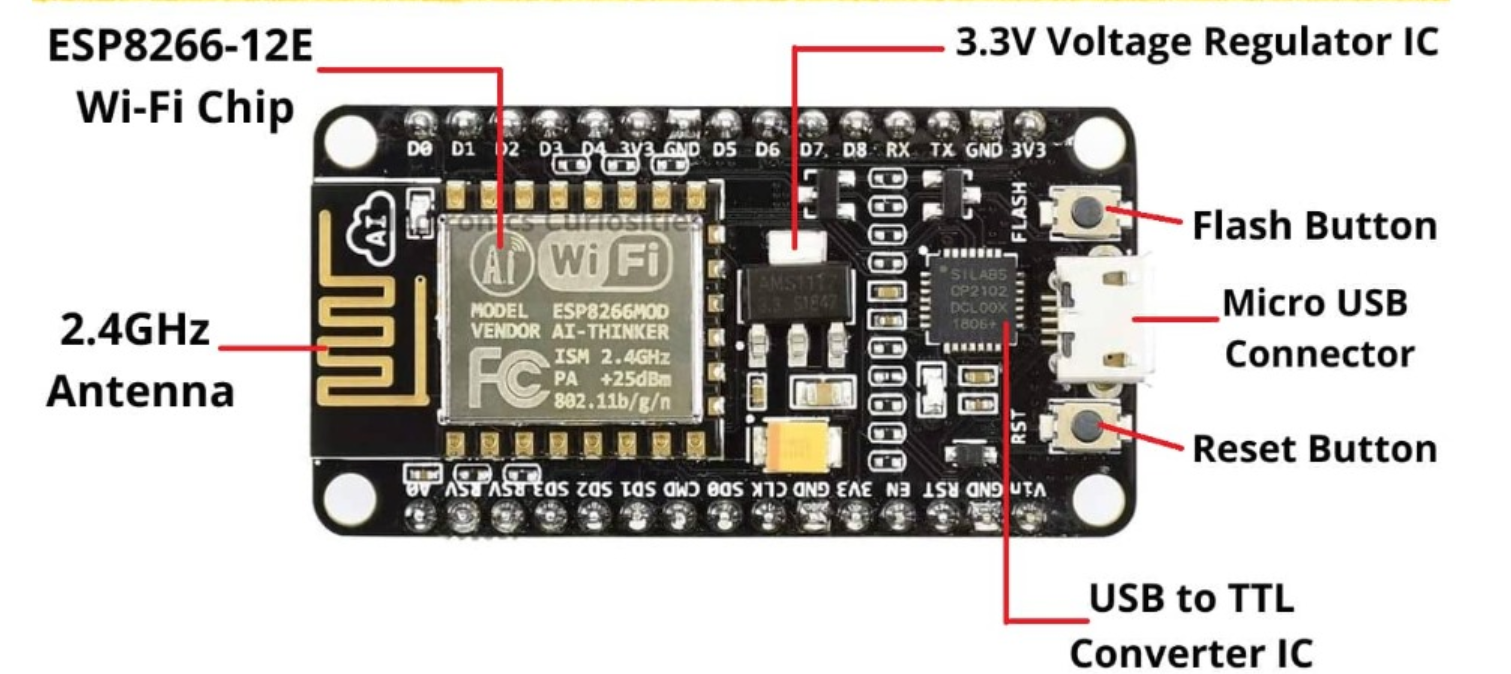
\includegraphics[width=0.8\linewidth]{C_chap/fig2.png}
     \caption{ ESP 8266}
 \end{figure}
\begin{figure}[htbp]
     \centering
     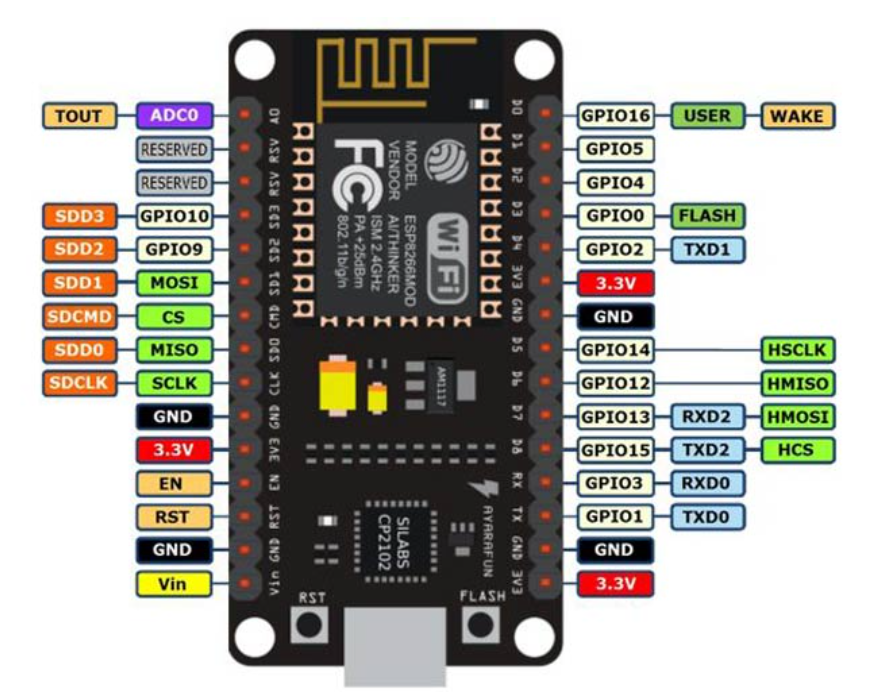
\includegraphics[width=0.8\linewidth]{C_chap/fig3.png}
     \caption{ ESP 8266 Pinout}
 \end{figure}
\subsection{AD 8232}
The AD8232 is a single-lead, heart rate monitoring analog front-end (AFE) integrated circuit designed by Analog Devices for applications in portable ECG (electrocardiogram) devices and heart rate monitors. This highly integrated chip includes instrumentation amplifiers, right-leg drive amplifiers, lead-off detection, and pace detection circuitry to provide a complete solution for biopotential signal acquisition. The device offers high input impedance, low input bias current, and low input-referred noise, ensuring accurate and reliable signal acquisition from the body. Its flexible design accommodates various electrode configurations and provides adjustable gain to optimize signal quality. The AD8232 operates from a single power supply, making it suitable for battery-powered applications. With its small form factor, low power consumption, and robust performance, the AD8232 simplifies the design of portable ECG devices and enables accurate heart rate monitoring in wearable health and fitness applications.
The healthcare industry has developed IoT real-time monitoring that allows doctors and specialists to diagnose patients quickly, smartly and effectively. Although there are many researches and studies that have developed methods for remote monitoring of ECG signals, the methods for monitoring and distributing these signals have not yet been agreed upon, so the process must be used to create complete health. Distribute the ECG signal. In this paper, we propose an ECG monitoring and classification. The application process is based on the communication of AD8232 sensor and ardunino node MCU, analog to digital converter and output ECG signal, which is used to convert the signal into a higher signal, and then send the output signal to the signal.Cloud-to-cloud use anywhere, the signal is pre-processed to remove the noise and QRS complex\cite{morshedlou2021ultra} is detected to determine the other characteristics of the signal such as heart rate, also to determine one cycle of ECG signal, later the signal is classified by using proposed  convolution neural network model  to detect the signal status. The extracted ECG signal is transmitted in real time to cloud (Ubidots cloud is used) through ESP8266 over to the cloud using WiFi based on MQTT publishing method. The experimental results are performed on different signals and the different stage of de-noising and QRS detection are applied and  different pooling layers are used in the proposed CNN model\cite{marriwala2023hybrid}.  The results show that the proposed classification model achieve accuracy up to 94\%.
he basic components of AD8232 are:
\\
\textbf{1. Instrumentation Amplifiers:}
\\
An instrumentation amplifier is a specialized type of operational amplifier\cite{dimas2022classification} (op-amp) configuration designed to amplify small differential signals while rejecting common-mode noise. It typically consists of three op-amps configured in a differential amplifier topology, with additional resistors for precise gain control. The primary function of an instrumentation amplifier is to amplify the voltage difference between two input signals while attenuating any common-mode signals present at both inputs. This allows for accurate measurement of small differential signals, making instrumentation amplifiers widely used in applications such as sensor interfacing, data acquisition systems, and medical instrumentation, where precision and noise rejection are paramount.
\\
\textbf{2. Right Leg Drive: }
\\
Right leg drive (RLD) is a technique commonly employed in biomedical instrumentation, particularly in electrocardiography\cite{noor2021predicting} (ECG) systems, to reduce common-mode interference and enhance the quality of acquired signals. In RLD, an electrode is placed on the patient's right leg and connected to the ground of the amplifier circuitry. By doing so, the common-mode voltage at the patient's body surface, including both the left and right arms, is shifted or driven towards the right leg. This effectively creates a reference point at the right leg, helping to cancel out common-mode noise picked up by the body. RLD is crucial in ECG systems as it improves the signal-to-noise ratio and minimizes artifacts, resulting in clearer and more accurate ECG recordings, particularly in environments prone to electrical interference.
\\
\textbf{3. Lead-Off Detection Circuitry:}
\\
Lead-off detection is a crucial feature in biomedical instrumentation, especially in electrocardiography (ECG) systems, aimed at ensuring the quality and reliability of the acquired signals. Lead-off detection identifies instances where the electrodes lose contact with the patient's skin or when the impedance between the electrode and the skin becomes too high, indicating a potential issue with signal acquisition. When lead-off is detected, it triggers an alert or warning, notifying the user or system operator of the problem. This feature is essential for maintaining the integrity of physiological measurements and preventing erroneous interpretations of data due to poor electrode contact or signal loss. Lead-off detection is often implemented using dedicated circuitry or algorithms that continuously monitor the electrical impedance at each electrode site, promptly identifying any abnormalities and allowing for timely corrective action to be taken.
\\
\textbf{4. Single Power Supply Operation: }
\\
The AD8232 is a single-lead electrocardiogram (ECG) analog front-end (AFE) integrated circuit (IC) manufactured by Analog Devices. One of its notable features is its ability to operate from a single power supply, which simplifies system design and reduces the overall component count required for building ECG monitoring systems. This characteristic is particularly advantageous for portable or wearable applications where space and power efficiency are critical considerations. By eliminating the need for dual power supplies, the AD8232 streamlines the design process, reduces system complexity, and lowers manufacturing costs. Additionally, operating from a single power supply enhances the versatility and ease of integration of the AD8232 into various ECG monitoring devices,becoming a popular choice among designers and engineers healthcare and wellness industries.
\\
\textbf{5. Low Input-Referred Noise: }
\\
"Low input-referred noise" refers to the minimal level of electrical noise introduced by an electronic device, such as an amplifier or sensor, at its input. In the context of biomedical instrumentation like electrocardiography (ECG), this term is particularly relevant as it pertains to the quality of the acquired physiological signals.
For instance, in an ECG system, low input-referred noise means that the amplifier used to capture the heart's electrical signals\cite{ksibi2023electroencephalography} introduces minimal additional noise to the signal being measured. This is crucial because ECG signals are typically very small in amplitude, measured in millivolts, and any additional noise can distort the signal, leading to inaccurate readings or difficulty in interpreting the data.
A low input-referred noise level ensures that the acquired signals maintain high fidelity and accuracy, allowing for reliable diagnosis and monitoring of cardiac activity. Achieving low input-referred noise often involves careful design considerations, including the use of high-quality components, proper shielding techniques, and optimized circuit layouts.
\\
\textbf{6. Flexible Input Configuration:}
\\
Firstly, the AD8232 can accommodate both single-lead and multi-lead ECG configurations. Single-lead configurations are commonly used in portable or wearable devices for basic heart rate monitoring, while multi-lead configurations, such as the standard 12-lead ECG, are utilized for more detailed cardiac assessments in clinical settings. The AD8232's adaptability to different lead configurations to ensure widespread use of monitoring scenarios, from basic health and wellness applications to medical diagnostics.
Moreover, the AD8232 is compatible with various types of electrodes, including disposable electrodes with adhesive gel, reusable electrodes with snap connectors, and dry electrodes with conductive materials. This compatibility enables users to choose the most suitable electrode type for their specific application requirements, considering factors such as comfort, convenience, and signal quality. Additionally, the AD8232's adjustable gain settings and integrated right-leg drive feature further enhance its versatility, allowing users to optimize signal acquisition for different electrode types and placements.
\\
\textbf{7. Built-in Filters:}
\\
The AD8232 includes built-in filters designed to enhance the quality of electrocardiogram (ECG) signal acquisition by mitigating noise and interference. These filters are integral to the analog front-end (AFE) circuitry of the AD8232 and serve to remove unwanted signals while preserving the desired ECG waveform \cite{pons2021evanescent}.
One of the primary filters incorporated into the AD8232 is a configurable low-pass filter. This filter attenuates high-frequency noise and artifacts that may be present in the ECG signal due to sources such as electromagnetic interference (EMI) or muscle activity. By selectively filtering out high-frequency components, the low-pass filter helps to improve the signal-to-noise ratio and enhance the clarity of the ECG waveform.
Additionally, the AD8232 may include other filters such as a high-pass filter to remove baseline drift and DC offset, as well as notch filters to suppress specific frequencies of interference, such as powerline noise (50 Hz or 60 Hz). These filters work synergistically to ensure that the acquired ECG signal is clean and free from common sources of distortion or interference.
\\
\\
\textbf{8. Small Form Factor:}
\\
The AD8232 is indeed engineered in a compact form factor, which significantly enhances its suitability for portable and wearable applications across various industries, particularly in healthcare and wellness. Its small size and lightweight design make it highly conducive for integration into a wide range of devices, including fitness trackers, wearable monitors, and portable medical devices.
The compact form factor of the AD8232 enables manufacturers to design sleek and unobtrusive wearable devices that can be comfortably worn by users throughout the day. Whether incorporated into wrist-worn fitness trackers or chest strap heart rate monitors, the AD8232's compact size ensures that the wearable device remains discreet and inconspicuous, promoting user comfort and convenience.
Additionally, the small footprint of the AD8232 facilitates the development of portable medical devices for ECG monitoring\cite{serhani2020ecg} applications. By integrating the AD8232 into handheld or handheld devices, healthcare professionals can conveniently perform on-the-go ECG monitoring, enabling timely diagnosis and intervention for patients in various settings such as clinics, ambulances, or remote locations.
Moreover, the compact size of the AD8232 allows for efficient use of space within the device, leaving room for other essential components such as batteries, microcontrollers\cite{daisy2021early}, and display screens. This optimization of space ensures that portable and wearable devices equipped with the AD8232 can offer comprehensive functionality while maintaining a sleek and ergonomic design.



 \begin{figure}[htbp]
    \centering
     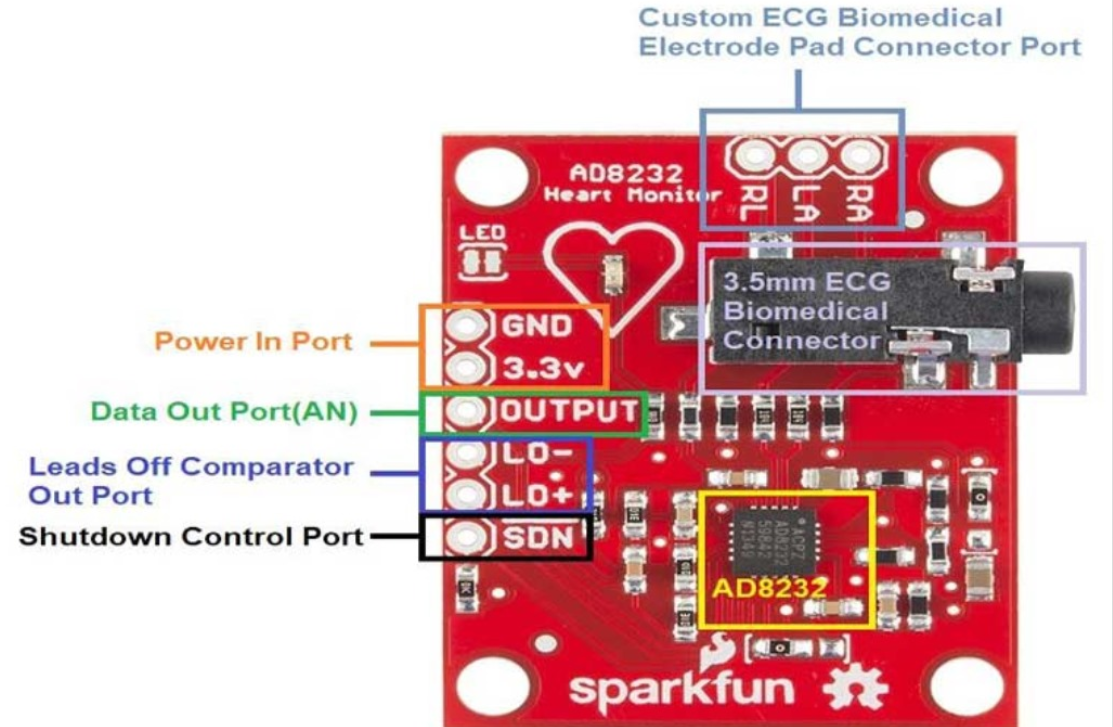
\includegraphics[width=0.7\linewidth]{C_chap/fig4.png}
\\\caption{ AD 8232}
 \end{figure}

\subsection{ECG Electrode}
Electrocardiogram (ECG) electrodes \cite{arquilla2020textile} are essential components used in biomedical instrumentation for capturing the electrical activity of the heart. These electrodes are typically placed on the patient's skin at specific locations to detect the electrical signals generated by the heart's contractions. ECG electrodes come in various forms, including disposable adhesive electrodes, reusable electrodes with snap connectors, and dry electrodes with conductive materials. They function by establishing electrical contact between the patient's skin and the monitoring device, allowing for the transmission of bioelectrical signals to the sensor or amplifier. ECG electrodes must adhere securely to the skin to ensure reliable signal acquisition and minimize motion artifacts, while also being gentle enough to prevent skin irritation or discomfort. Overall, ECG electrodes\cite{roh2014wearable} play a crucial role in obtaining accurate and reliable ECG readings, making them indispensable components in healthcare settings for diagnostic, monitoring, and research purposes. Here are the details of each component of an ECG electrode:

\textbf{1. Adhesive Patch/Pad:}
    Adhesive patches or pads are specialized types of electrodes commonly used in electrocardiogram (ECG) monitoring and other biomedical applications. These electrodes are designed with an adhesive backing that allows them to securely adhere to the patient's skin, ensuring reliable contact and signal acquisition throughout the monitoring period. Adhesive patches or pads are particularly advantageous for long-term monitoring or ambulatory ECG recordings, as they provide a stable and comfortable attachment that minimizes the risk of electrode displacement or motion artifacts.
    These electrodes come in various shapes and sizes, including rectangular patches, circular pads, or custom-shaped designs, to accommodate different electrode placements and patient preferences. They are typically equipped with conductive gel or solid conductive materials to facilitate the transmission of electrical signals from the patient's skin to the monitoring device. Adhesive patches or pads are also available in disposable or reusable options, depending on the specific application requirements and cost considerations.

\textbf{2. Conductive Gel:}
    Conductive gel is a specialized substance used in conjunction with electrodes in biomedical applications, particularly in electrocardiography (ECG) and electromyography (EMG) \cite{merletti2020tutorial}. It serves as an interface between the skin and the electrode, facilitating the transmission of electrical signals while minimizing impedance and improving signal quality.Conductive gel is typically water-based and contains electrolytes to enhance conductivity. When applied to the skin beneath the electrode, it helps to reduce the skin-electrode interface impedance by filling in microscopic irregularities and ensuring uniform contact. This results in a more reliable and stable electrical connection, leading to clearer and more accurate recordings of physiological signals.
    In addition to improving signal quality, conductive gel also serves to protect the skin from irritation or discomfort caused by prolonged contact with electrodes. It is formulated to be non-drying and hypoallergenic, Made suitable for use by many patients, including those with sensitive skin.

\textbf{3. Connector:}
   Connectors play a critical role in biomedical instrumentation by facilitating the secure and reliable connection between various components, such as electrodes, cables, sensors, and monitoring devices. In electrocardiogram (ECG) monitoring, connectors are used to link the electrodes to the monitoring equipment, ensuring the transmission of electrical signals with minimal interference or signal loss.There are several types of connectors commonly used in biomedical applications, including snap connectors, banana plugs, and DIN connectors. Snap connectors are often found on disposable or reusable ECG electrodes, providing a quick and easy way to attach and detach the electrodes from the monitoring device. Banana plugs, with their simple and robust design, are commonly used for connecting cables to ECG machines or amplifiers. DIN connectors, characterized by their circular shape and multiple pins, are used in more specialized applications where additional functionalities or signal channels are required.
   Connectors are designed with features such as locking mechanisms, shielding, and insulation to ensure a secure and stable connection while minimizing the risk of signal interference or electrical hazards. Additionally, connectors may be color-coded or labeled to facilitate proper alignment and orientation during assembly, reducing the likelihood of errors and ensuring compatibility between components..

\textbf{4. Lead Wire:}
      Lead wires are essential components in biomedical instrumentation, particularly in electrocardiography (ECG) and other physiological monitoring systems. These wires serve as conduits for transmitting electrical signals between electrodes placed on the patient's body and the monitoring device or amplifier.
      Lead wires are typically made of flexible and durable materials such as insulated copper or silver conductors, allowing for easy maneuverability and reliable signal transmission without compromising patient comfort. They come in various lengths to accommodate different electrode placements and patient sizes, ranging from short lengths for limb electrodes to longer lengths for chest or back electrodes. Lead wires are equipped with connectors on both ends to facilitate secure and standardized connections between electrodes and monitoring equipment. These connectors may include snap connectors, banana plugs, or DIN connectors\cite{libman2023ecg}, depending on the specific requirements of the monitoring system and the type of electrodes being used.In addition to transmitting electrical signals, lead wires may also feature color-coded markings or labeling to facilitate proper electrode placement and connection, reducing the risk of errors during setup. Some lead wires may also incorporate shielding or insulation to minimize the risk of electromagnetic interference and ensure the integrity of the transmitted signals.

\textbf{5. Electrode Size and Shape:}
       Electrodes used in biomedical applications come in various sizes and shapes to accommodate different patient populations and electrode placements. Standard sizes for adult electrodes often range from 1 inch (2.5 cm) to 1.5 inches (3.8 cm) in diameter. Circular and oval shapes are common due to their versatility and ease of application, allowing for consistent contact with the skin. However, rectangular or square-shaped electrodes are also available and may be preferred for specific electrode placements or applications where a larger surface area is required.In addition to standard sizes for adults, pediatric electrodes are available in smaller sizes to suit the anatomical dimensions of infants and small children. These electrodes are typically designed with reduced diameters and may feature specialized shapes or designs to ensure optimal skin contact and comfort for pediatric patients.
       The selection of electrode size and shape depends on various factors, including the patient's age, body size, and the specific monitoring application. Healthcare professionals carefully consider these factors when choosing the appropriate electrodes to ensure accurate signal acquisition and patient comfort during diagnostic or monitoring procedures. Overall, the availability of electrodes in different sizes and shapes enhances the versatility and effectiveness of biomedical instrumentation across diverse patient populations and clinical settings.

\textbf{6. Pre-gelled vs Dry Electrodes:}
         Pre-gelled electrodes come pre-coated with a conductive gel or adhesive gel layer, which enhances electrical conductivity and ensures optimal skin contact upon application. These electrodes are convenient to use, as they eliminate the need for separate gel application and reduce preparation time during electrode placement. Pre-gelled electrodes are particularly advantageous for quick and easy setup in clinical settings where efficiency is crucial. They also help to minimize skin irritation or discomfort during prolonged monitoring sessions by providing a smooth and cushioned interface between the electrode and the skin.On the other hand, dry electrodes do not require any conductive gel or adhesive gel layer and rely on dry contact with the skin for signal acquisition. Instead of gel, dry electrodes utilize specialized materials or surface treatments to promote conductivity and maintain stable skin-electrode contact. Dry electrodes offer the advantage of being mess-free and non-sticky, making them more comfortable for patients, especially those with sensitive skin or allergies to gel ingredients. Additionally, dry electrodes are reusable and do not require frequent replacement, leading to cost savings over time.
         The choice between pre-gelled and dry electrodes depends on various factors, including the specific monitoring application, patient preferences, and clinical requirements. While pre-gelled electrodes offer convenience and immediate readiness, dry electrodes provide a comfortable and cost-effective alternative for long-term monitoring or patients with skin sensitivities. Healthcare professionals carefully consider these factors when selecting the most suitable type of electrode for each patient and clinical scenario, ensuring optimal signal quality and patient comfort during diagnostic or monitoring procedures.

\textbf{7. Disposable vs Reusable:}
         Disposable and reusable electrodes are two types of electrodes commonly used in biomedical applications for electrocardiography (ECG), Electromyography\cite{schwartz1978facial} (EMG), and other physiological monitoring systems. Each type has distinct characteristics and advantages, catering to different clinical needs and preferences.
         Disposable electrodes are designed for single-use applications and are intended to be discarded after a single patient interaction or monitoring session. These electrodes typically come gelled or attached with a conductive gel layer, eliminating the need for additional gel application and reducing setup time. Disposable electrodes offer convenience and hygiene benefits, as they help prevent cross-contamination between patients and reduce the risk of infection transmission in clinical settings. They are particularly suitable for short-term monitoring applications, such as emergency care, ambulatory monitoring, or routine diagnostic tests.
        On the other hand, reusable electrodes are designed for multiple uses and can be cleaned and sterilized between patient interactions. These electrodes are typically made of durable materials such as metal or plastic and may require separate gel application before each use. Reusable electrodes offer cost-effectiveness and environmental benefits, as they can be used repeatedly over an extended period, reducing waste and lowering overall healthcare costs. They are well-suited for long-term monitoring applications, such as inpatient care, outpatient clinics, or home healthcare settings, where frequent electrode replacement may not be feasible or economical.

\textbf{8. Electrode Placement:}
    Electrode placement is a critical aspect of electrocardiogram (ECG) monitoring, ensuring accurate signal acquisition and interpretation. Standardized locations are designated for each electrode based on the standard ECG lead system, which includes limb leads and chest leads. Limb leads are typically placed on the arms and legs, while chest leads are positioned on the chest wall \cite{pesti2020electrode} .Color coding is commonly used to match electrodes with their corresponding leads, facilitating accurate placement by healthcare providers. For example, electrodes for limb leads may be color-coded with red for the right arm, yellow for the left arm, green for the right leg, and black for the left leg. Similarly, chest electrodes are often color-coded to correspond with specific chest lead positions, such as V1 through V6.
    By adhering to standardized electrode placement and color coding, healthcare providers can ensure consistency and accuracy in ECG monitoring procedures. This not only streamlines the process of electrode application but also helps to prevent errors and misinterpretations of ECG data. Standardized placement and color coding contribute to the efficiency and reliability of ECG monitoring, ultimately enhancing patient care and diagnostic accuracy.

\textbf{9. Compatibility:}
         Compatibility is a crucial aspect of ECG electrodes, ensuring seamless integration with lead wires and compatibility with a wide range of ECG machines. Modern ECG electrodes often feature universal connectors designed to fit standard ECG lead wires commonly used in clinical settings. These universal connectors provide a standardized interface, allowing electrodes to be easily connected and disconnected from lead wires without the need for specialized adapters or connectors.Furthermore, ECG electrodes are designed to be compatible with a variety of ECG machines from different manufacturers. This compatibility ensures that healthcare providers have flexibility in choosing the appropriate electrodes for their specific monitoring equipment, regardless of the brand or model. Whether used with portable handheld devices, bedside monitors, or advanced diagnostic systems, ECG electrodes are engineered to deliver reliable signal acquisition and compatibility across diverse ECG machine platforms.
        By offering universal connectors and compatibility with a wide range of ECG machines, ECG electrodes facilitate efficient and interoperable monitoring procedures in clinical environments. Healthcare providers can confidently select electrodes that meet their performance and compatibility requirements, ensuring optimal signal quality and patient care during ECG monitoring and diagnostic procedures.

\textbf{10. Hygiene and Storage:}
         Proper hygiene and storage are essential to maintain the integrity and performance of ECG electrodes throughout their shelf life.To ensure optimal hygiene and prevent contamination, ECG electrodes are often individually packaged in hygienic packaging materials. This packaging helps maintain sterility and prevents exposure to environmental contaminants, ensuring that the electrodes are clean and safe for use in clinical settings.Additionally, proper storage conditions are essential for preserving the quality of ECG electrodes. Electrodes should be stored in a cool, dry place away from direct sunlight, as exposure to heat and moisture can degrade the electrode materials and compromise their performance. Storing electrodes in a controlled environment helps prevent the gel from drying out or the adhesive from losing its effectiveness over time, ensuring that the electrodes maintain their adhesive properties and conductivity for reliable signal acquisition.
         By adhering to hygienic packaging practices and proper storage guidelines, healthcare providers can ensure that ECG electrodes remain clean, sterile, and effective for use in patient monitoring and diagnostic procedures. This helps uphold the highest standards of patient safety and quality of care in clinical environments.

 \begin{figure}[htbp]
    \centering
     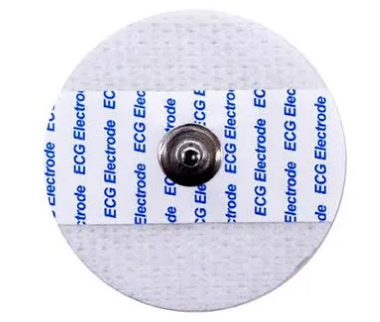
\includegraphics[width=0.7\linewidth]{C_chap/fig5.png}
\\\caption{ ECG Electrode}
 \end{figure}

\section{Block Diagram of project}

\textbf{1. ECG Leads:}
\begin{itemize}
    \item An ECG lead is an electrical conductor that connects the body to an electrocardiogram (ECG) machine, facilitating the measurement and recording of the heart's electrical activity. These leads are essential components of ECG monitoring systems, providing valuable insights into the heart's rhythm, rate, and conduction pathways. There are two main types of ECG leads: limb leads and chest leads. Limb leads are placed on the limbs of the body and record the electrical activity in the frontal plane, while chest leads, also known as precordial leads, are positioned on the chest wall to capture the electrical activity in the horizontal plane. By analyzing the signals obtained from these leads, healthcare professionals can diagnose various cardiac conditions, monitor the effectiveness of treatments, and assess the overall function of the heart, contributing to the management of cardiovascular health.
\end{itemize}

\textbf{2. AD8232 Sensor:}
\begin{itemize}
    \item The AD8232 sensor \cite{mendes2023ad8232} is a highly integrated, single-lead electrocardiogram (ECG) front-end module designed for monitoring cardiac electrical activity in portable and wearable devices. This compact and versatile sensor incorporates essential components such as instrumentation amplifiers, lead-off detection circuitry, and right leg drive (RLD) amplifiers\cite{yang2021new}, providing high-quality ECG signal acquisition while minimizing power consumption. The AD8232 sensor features a low-pass filter to attenuate noise and interference, ensuring accurate ECG signal capture even in noisy environments. Additionally, its built-in right leg drive circuitry helps reduce common-mode interference and improve common-mode rejection ratio, enhancing the signal-to-noise ratio of the acquired ECG signals. With its small form factor, low power consumption, and robust performance, the AD8232 sensor is The AD8232 sensor is ideal for a variety of medical and healthcare applications including remote patient monitoring, security monitoring and Holter monitoring..
\end{itemize}

\textbf{3. ESP8266 (WiFi Module):}
\begin{itemize}
    \item The ESP8266 is a highly versatile and compact WiFi module developed by Espressif Systems, renowned for its affordability, simplicity, and robust performance. Integrating a powerful 32-bit microcontroller unit (MCU) with a built-in WiFi radio transceiver, the ESP8266 enables seamless wireless connectivity for a diverse range of embedded applications. Supporting IEEE 802.11 b/g/n WiFi standards, the module facilitates easy integration into WiFi networks, allowing devices to communicate with each other and connect to the Internet. With its extensive GPIO pins \cite{schmidli2023different}, native TCP/IP protocol stack, and low-power consumption features, the ESP8266 serves as a versatile platform for developing devices, home automation systems, smart appliances, and DIY electronics projects, It is becoming a popular choice among hobbyists, developers and professional developers.
\end{itemize}

\textbf{4. UbidotS (Cloud Service):}
\begin{itemize}
   \item The ESP8266 module sends the processed ECG data to the Ubidots cloud service.
   Data Storage and Processing: Ubidots receives, stores, and processes the ECG data in the cloud.
  It provides a platform for real-time data visualization, analysis, and monitoring.
\end{itemize}
\textbf{5. Ubidots App :}
\begin{itemize}
   \item Ubidots is a leading cloud-based Internet of Things (IoT) platform that empowers users to easily collect, store, visualize, and analyze sensor data in real-time. With its intuitive interface and comprehensive suite of features, Ubidots enables users to build scalable IoT applications and solutions quickly and efficiently. From data collection and storage to visualization and analysis, Ubidots provides a seamless end-to-end solution for IoT development and deployment. Its ordered dashboards, powerful analytics tools, and integration options allow users to gain valuable insights from their IoT data and drive informed decision-making. Whether for industrial monitoring, environmental sensing, smart cities, or consumer IoT applications, Ubidots provides the tools and capabilities needed to Unleash the full potential of IoT and drive innovation across industries and markets.
\end{itemize}


 \begin{figure}[htbp]
    \centering
     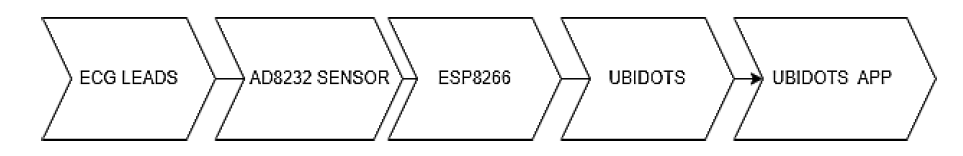
\includegraphics[width=1.1\linewidth]{C_chap/fig6.png}
\caption{ Block Diagram}
 \end{figure}

\begin{itemize}
    \item The patient's ECG signals are captured by the electrodes (ECG Leads).
\end{itemize}
\begin{itemize}
    \item The AD8232 Sensor processes these signals, making them suitable for digital processing.
\end{itemize}
\begin{itemize}
    \item The ESP8266 module establishes a wireless connection to the internet and sends the processed ECG data to the Ubidots cloud service.
\end{itemize}
\begin{itemize}
    \item Ubidots stores, analyzes, and visualizes the ECG data in real-time on its platform.
\end{itemize}
\begin{itemize}
    \item The Ubidots app, accessible through web or mobile devices, provides a user-friendly interface for monitoring the patient's ECG graphs and vital statistics.
\end{itemize}
This project enables continuous, real-time monitoring of a patient's ECG signals remotely. Healthcare providers or caregivers can access the Ubidots app to keep track of the patient's heart health, receive alerts for any abnormalities, and take necessary actions promptly.

 \begin{figure}[htbp]
    \centering
     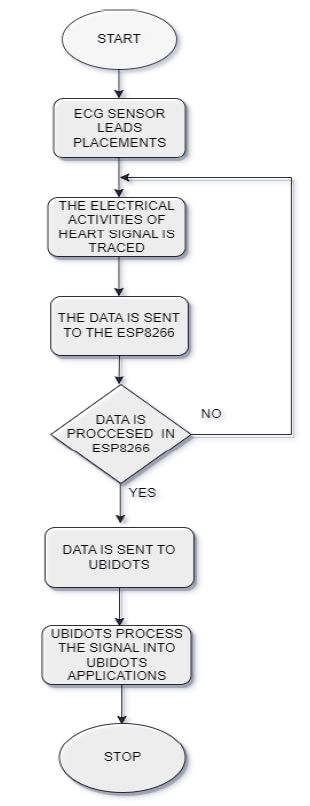
\includegraphics[width=0.6\linewidth]{C_chap/fig7.png}
\caption{ Process Flow}
 \end{figure}
\section{Experimental Configuration}
 We've designed a system using three ECG leads to capture important aspects of the heart's electrical activity. Previous research suggests that this arrangement is enough to get the key details we need. The trick is to place the electrodes in a triangle shape around the heart, as shown in Figure 1 of our system. We wanted to make sure our system is both stable and accurate, so we tested it on a healthy volunteer. This volunteer wore the three electrodes in the triangle setup while doing different activities. The system worked well, showing clear heart rate changes and waveform patterns during rest, light exercise, and deep breathing. This setup seems promising for keeping an eye on heart health, especially in everyday settings. The next step? We plan to test it with more people to see how well it works for different folks.
\\
Typical ECG signals are made up of five types of waves:
P surge, T surge, Q surge, R surge, and S surge. These waves intervals are commonly utilised to diagnose a number of heart conditions. Among all the features of these waves, four are most commonly used in medical diagnosis.
 \begin{figure}[htbp]
    \centering
     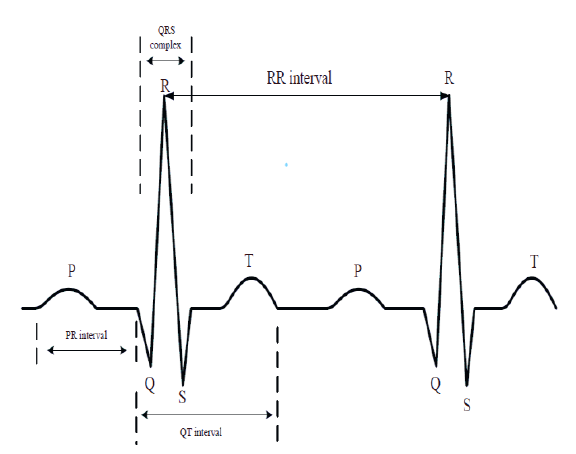
\includegraphics[width=0.9\linewidth]{C_chap/fig8.png}
\\\caption{Standard ECG Signal}
 \end{figure}
\begin{itemize}
    \item \textbf{RR Break:} The RR break, also known as the RR interval, is a crucial measure in analyzing an ECG signal, particularly because it signifies the time between two consecutive R waves. The R wave, being a prominent feature of the ECG waveform, is often used as a reference point due to its consistency and clear identification. The RR interval reflects the heart's rhythm, with variations indicating irregularities that might signal underlying heart condition\cite{arquilla2020textile}. By measuring the duration between R waves, healthcare providers can assess the regularity and stability of the heart's electrical activity. In cases of arrhythmia or other cardiac abnormalities, the RR interval may show irregular patterns, providing valuable diagnostic information for appropriate medical intervention.
\end{itemize}
\begin{itemize}
    \item \textbf{PR Break:} The PR break, known as the PR interval, is a fundamental component of an ECG signal, indicating the time between the beginning of the P wave and the start of the QRS complex. This interval provides insight into the conduction time from the atria (upper chambers of the heart) to the ventricles (lower chambers). Essentially, it measures the duration it takes for the electrical impulse generated by the sinoatrial (SA) node to travel through the atria, pass through the atrioventricular (AV) node, and reach the ventricles to trigger their contraction. A normal PR interval reflects a healthy electrical conduction system, ensuring coordinated heart contractions. Deviations from the normal range can indicate conditions such as heart block, where the impulse is delayed or blocked in its path, affecting the heart's rhythm and efficiency. Monitoring the PR interval helps clinicians assess the integrity of the heart's electrical pathways and identify potential cardiac abnormalities.
\end{itemize}
\begin{itemize}
    \item \textbf{QT Break:} The QT break, referred to as the QT interval, is a critical measure on an ECG representing the time from the beginning of the Q wave to the end of the T wave. This interval signifies the duration of both ventricular depolarization (contraction) and relaxation of the heart. It reflects the time it takes for the heart's electrical activity to stimulate the ventricles to contract and then recover to their resting state. A normal QT interval indicates proper coordination and timing of these electrical events. However, if the QT interval extends beyond its expected value, it may indicate a higher risk of ventricular arrhythmias, such as ventricular fibrillation. Ventricular fibrillation is a dangerous and potentially life-threatening condition where the heart's rhythm becomes chaotic, leading to inadequate blood flow and sudden cardiac arrest. Monitoring the QT interval is crucial in assessing the risk of these serious cardiac events, guiding clinicians in preventive measures and appropriate treatment strategies.
    \item \textbf{QRS Break:} The QRS break, or the QRS complex, is a key component of an ECG signal that reflects the electrical activity during ventricular depolarization, the phase when the ventricles contract. It consists of three main waves: the Q wave, the R wave (the largest deflection), and the S wave. The QRS complex represents the rapid spread of electrical impulses through the ventricles, leading to their contraction and the ejection of blood from the heart. Analyzing the shape, duration, and amplitude of the QRS complex provides valuable information about the heart's health and function. Certain conditions, such as electrolyte imbalances or drug toxicities, can manifest as changes in the QRS complex. For example, an enlarged QRS complex might indicate a blockage in the heart's electrical pathways, while a widened or prolonged QRS complex could suggest conditions like bundle branch blocks. These insights help clinicians diagnose and manage various cardiac disorders, allowing for timely interventions and appropriate treatment plans.
\end{itemize}
\section{Key Challenges of ECG Monitoring System}
The ECG monitoring systems, as discussed in this paper, are constructed from a diverse array of components, frameworks, and technologies. This diversity and heterogeneity in ECG sensor-based architectures present several challenges, as highlighted by numerous researchers in the field. A multitude of obstacles can arise, including interoperability issues between different sensor types and data formats. The integration of various sensors and devices into a cohesive system can pose technical complexities, leading to compatibility issues and difficulties in data synchronization. Furthermore, the management More ECG data, often generated on the fly, requires robust storage solutions and efficient data processing mechanisms. Additionally, ensuring the security and privacy of sensitive patient data in these systems remains a paramount concern. Addressing these challenges necessitates collaborative efforts among researchers, engineers, and healthcare professionals to develop standardized protocols, seamless integration frameworks, and robust data management strategies for reliable and effective ECG monitoring systems \cite{serhani2020ecg}.
\\
There are a variety of obstacles that can be encountered, including the following:
\\
\textbf{1. Signal Quality Issues:}
One of the primary challenges with ECG monitoring devices is ensuring consistent and reliable signal quality.
Factors such as poor electrode contact with the skin, motion artifacts, and external interference can degrade the signal.
These issues can lead to inaccuracies in the recorded ECG data, making it challenging to obtain precise diagnostic information.
\\
\textbf{2. Difficulties with Durability Monitoring:}
Monitoring devices, especially those used in ambulatory or continuous monitoring settings, need to withstand daily wear and tear.
Durability becomes crucial to ensure that the devices remain functional and accurate over extended periods.
Factors such as battery life, water resistance, and robustness against physical damage are key considerations.
\\
\textbf{3. Issues with the Size of ECG Signal Data:}
ECG signals generate a significant amount of data, especially in continuous monitoring applications.
Storing and managing these large datasets pose challenges in terms of storage capacity and data transfer.
Efficient compression techniques and optimized data transmission protocols are essential to handle the sizeable ECG signal data efficiently.
\\
\textbf{4. Visualization-Related Difficulties:}
Interpreting ECG graphs and trends is critical for healthcare providers to make accurate diagnoses and treatment decisions.
However, the complexity of ECG data visualization, especially in real-time monitoring, can be a challenge.
Clear and intuitive graphical representations are needed to convey information effectively without overwhelming the user.
\\
\textbf{5. Difficulties with System Integration:}
ECG monitoring devices often need to integrate with other healthcare systems, such as Electronic Health Records (EHR) or platforms.
Achieving seamless integration requires compatibility with different data formats, communication protocols, and interoperability standards.
Ensuring that data from ECG devices can be easily shared, accessed, and analyzed within broader healthcare systems is crucial for efficient patient care.
\section{Addressing the Challenges}
\textbf{1. Signal Quality Enhancement:}
Advanced signal processing algorithms can help mitigate noise and artifacts in ECG signals, improving overall signal quality.
Use of high-quality electrodes and proper skin preparation techniques can enhance electrode-skin contact, reducing signal interference.
\\
\textbf{2. Improved Device Durability:}
Designing monitoring devices with robust materials and construction can enhance durability.
Incorporating features such as waterproofing, shock resistance, and long-lasting batteries improves device reliability.
\\
\textbf{3. Efficient Data Management:}
Employing data compression algorithms and cloud-based storage solutions can address the challenges of large ECG signal datasets.
Implementing data encryption and secure transmission protocols ensures data security and privacy.
\\
\textbf{4. Enhanced Visualization Tools:}
Developing user-friendly interfaces with intuitive ECG waveform displays aids healthcare providers in interpreting data effectively.
Real-time trend analysis and alarm systems can help highlight abnormalities for timely intervention.
\\
\textbf{5. Interoperability and System Integration:}
Adhering to standard data formats such as HL7 (Health Level Seven) or DICOM (Digital Imaging and Communications in Medicine) promotes interoperability.
Developing Application Programming Interfaces (APIs) and middleware solutions facilitate seamless integration with existing healthcare IT systems.
\\
By addressing these challenges through technological innovations, improved device design, and standardized protocols, ECG monitoring devices can become more reliable, user-friendly, and effective tools in the realm of healthcare, enabling better patient care and outcomes.
\\
Continuous remote monitoring through wireless connectivity options like Bluetooth or WiFi allows healthcare providers to track patients ECG signals in real-time, facilitating early detection of abnormalities and timely intervention. Personalized alert systems, tailored to individual patient profiles and medical history, ensure that relevant notifications are delivered promptly, enhancing patient management and outcomes. Integration of artificial intelligence (AI) algorithms enhances diagnostic accuracy and predictive capabilities by analyzing ECG data in real-time, aiding healthcare providers in making informed clinical decisions. Wearable form factors such as smartwatches or patches improve patient comfort and compliance with long-term monitoring protocols, enabling continuous monitoring during daily activities. E-medicine integration enables remote consultation and diagnosis, particularly beneficial in poor areas, enhancing access to specialized cardiac care and reducing healthcare disparities. Long-term data trends analysis tools track changes in patients cardiac health over time, guiding proactive treatment decisions based on subtle changes or collapse in cardiac function. Patient education materials and interactive features within ECG monitoring devices promote patient engagement and empowerment, leading to better adherence to treatment plans and improved health outcomes.
\pagebreak